\chapter{The EPK is a Kernel}

% \section{EPK Proof}
% \ker*
% \begin{proof}
% We must show that the associated kernel matrix $K_{\text{EPK}} \in \mathbb{R}^{n\times n}$ defined for an arbitrary subset of data $\{x_i\}_{i=1}^M \subset X$ as $K_{\text{EPK},i,j} = \int_0^1\langle \phi_{s,t}(x_i), \phi_{s,t}(x_j)\rangle dt$ is both symmetric and positive semi-definite.

% Since the inner product on a Hilbert space $\langle \cdot, \cdot \rangle$ is symmetric and since the same mapping $\varphi$ is used on the left and right, $K_{\text{EPK}}$ is \textbf{symmetric}. 

% To see that $K_{\text{EPK}}$ is \textbf{Positive Semi-Definite}, let $\alpha = (\alpha_1, \alpha_2, \dots, \alpha_n)^\top \in \mathbb{R}^n$ be any vector. We need to show that $\alpha^\top K_{\text{EPK}} \alpha \geq 0$. We have

% \begin{align}
% \alpha^\top K_{\text{EPK}} \alpha &= \sum_{i=1}^n \sum_{j=1}^n \alpha_i \alpha_j \int_0^1 \langle \phi_{s,t}(x_i), \phi_{s,t}(x_j)\rangle dt \\
% &= \sum_{i=1}^n \sum_{j=1}^n \alpha_i \alpha_j \int_0^1 \langle \nabla_{w}\hat{y}_{w_s(t,x_i)}, \nabla_{w}\hat{y}_{w_s(t,x_j)}\rangle dt \\
% &= \int_0^1 \sum_{i=1}^n \sum_{j=1}^n \alpha_i \alpha_j \langle \nabla_{w}\hat{y}_{w_s(t,x_i)}, \nabla_{w}\hat{y}_{w_s(t,x_j)}\rangle dt \\
% &= \int_0^1 \sum_{i=1}^n \sum_{j=1}^n  \langle \alpha_i \nabla_{w}\hat{y}_{w_s(t,x_i)}, \alpha_j \nabla_{w}\hat{y}_{w_s(t,x_j)}\rangle dt \\
% &= \int_0^1    \langle \sum_{i=1}^n \alpha_i \nabla_{w}\hat{y}_{w_s(t,x_i)}, \sum_{j=1}^n \alpha_j \nabla_{w}\hat{y}_{w_s(t,x_j)}\rangle dt \\
% & \text{Re-ordering the sums so that their indices match, we have}\\
% &= \int_0^1 \left\lVert \sum_{i=1}^n \alpha_i \nabla_{w}\hat{y}_{w_s(t,x_i)}\right\rVert^2 dt \\
% &\geq 0,
% \end{align}

% Note that this reordering does not depend on the continuity of our mapping function $\phi_{s,t}(x_i)$.

% \end{proof}

% \textbf{Remark \remlabel{rem2}} In the case that our mapping function $\varphi$ is not symmetric, after re-ordering, we still yield something of the form:
% \begin{align}
% &= \int_0^1 \left\lVert \sum_{i=1}^n \alpha_i \nabla_{w}\hat{y}_{w_s(t,x_i)}\right\rVert^2 dt \\
% \end{align}
% The natural asymmetric $\phi$ is symmetric for every non-training point, so we can partition this sum. For the non-training points, we have symmetry, so for those points we yield exactly the $L^2$ metric. For the remaining points, if we can pick a Lipschitz constant $E$ along the entire gradient field, then if training steps are enough, then the integral and the discrete step side of the asymmetric kernel will necessarily have positive inner product. In practice, this Lipschitz constant will change during training and for appropriately chosen step size (smaller early in training, larger later in training) we can guarantee positive-definiteness. In particular this only needs to be checked for training points. 

% \subsection{The EPK gives an Exact Representation}
% \label{proof:eker}
% \eker*
% \begin{proof}

% Let $f_{w}$ be a differentiable function parameterized by parameters $w$ which is trained via $N$ forward Euler steps of fixed step size $\varepsilon$ on a training dataset $X$ with labels $ Y$, with initial parameters $w_0$ so that there is a constant $b$ such that for every $x$, $f_{w_0}(x) = b$, and weights at each step ${w_s : 0 \leq s \leq N}$. Let $x \in X$ be arbitrary and within the domain of $f_w$ for every $w$. For the final trained state of this model $f_{w_N}$, let $y = f_{w_N}(x)$. 

% For one step of training, we consider $y_s  = f_{w_s(0)}(x)$ and $y_{s+1} = f_{w_{s+1}}(x)$. We wish to account for the change $y_{s+1} - y_s$ in terms of a gradient flow, so we must compute $\dfrac{\partial y}{dt}$ for a continuously varying parameter $t$. Since $f$ is trained using forward Euler with a step size of $\varepsilon > 0$, this derivative is determined by a step of fixed size of the weights $w_s$ to $w_{s+1}$. We parameterize this step in terms of the weights:

% \begin{align}
%     \dfrac{d w_s(t)}{dt} &= (w_{s+1} - w_s)\\   
%     \int \dfrac{d w_s(t)}{dt} dt &= \int (w_{s+1} - w_s)dt\\
%     w_s(t) &= w_s + t(w_{s+1} - w_s)\\
% \end{align}
% Since $f$ is being trained using forward Euler, across the entire training set $X$ we can write:
% \begin{align}
%     \dfrac{d w_s(t)}{dt} &= -\varepsilon \nabla_w L(f_{w_s(0)}(X), y_i) = -\varepsilon \sum_{j = 1}^{d} \sum_{i=1}^M  \dfrac{\partial L(f_{w_s(0)}(x_i),  y_i)}{\partial w_j} \label{eq10}
% \end{align}
% Applying chain rule and the above substitution, we can write
% \begin{align}
%     \dfrac{d \hat y}{dt} = \dfrac{d f_{w_s(t)}}{dt} &= \sum_{j = 1}^{d} \dfrac{d f}{\partial w_j} \dfrac{\partial w_j}{dt}\\
% &= \sum_{j = 1}^{d} \dfrac{d f_{w_s(t)}(x)}{\partial w_j} \left(-\varepsilon \dfrac{\partial L(f_{w_s(0)}(X_T),  Y_T)}{\partial w_j}\right)\\
% &= \sum_{j = 1}^{d} \dfrac{d f_{w_s(t)}(x)}{\partial w_j} \left(-\varepsilon \sum_{i = 1}^{M}\dfrac{d L(f_{w_s(0)}(x_i),  y_i)}{d f_{w_s(0)}(x_i)}\dfrac{\partial  f_{w_s(0)}(x_i)}{\partial w_j}\right)\\
% &= -\varepsilon \sum_{i = 1}^{M} \dfrac{d L(f_{w_s(0)}(x_i),  y_i)}{d f_{w_s(0)}(x_i)} \sum_{j = 1}^{d} \dfrac{d f_{w_s(t)}(x)}{\partial w_j}  \dfrac{d f_{w_s(0)}(x_i)}{\partial w_j}\\
% &= -\varepsilon \sum_{i = 1}^{M} \dfrac{d L(f_{w_s(0)}(x_i),  y_i)}{d f_{w_s(0)}(x_i)} \nabla_w f_{w_s(t)}(x) \cdot \nabla_w f_{w_s(0)}(x_i)\\
% \end{align}
% Using the fundamental theorem of calculus, we can compute the change in the model's output over step $s$
% \begin{align}
%     y_{s+1} - y_s &= \int_0^1 -\varepsilon \sum_{i = 1}^{M} \dfrac{d L(f_{w_s(0)}(x_i),  y_i)}{d f_{w_s(0)}(x_i)}  \nabla_w f_{w_s(t)}(x) \cdot \nabla_w f_{w_s(0)}(x_i)dt\\
%  &=  -\varepsilon \sum_{i = 1}^{M} \dfrac{d L(f_{w_s(0)}(x_i),  y_i)}{d f_{w_s(0)}(x_i)}  \left(\int_0^1\nabla_w f_{w_s(t)}(x)dt\right) \cdot \nabla_w f_{w_s(0)}(x_i)\\
% \end{align}
% For all $N$ training steps, we have
% \begin{align*}
% y_N &= b + \sum_{s=1}^N y_{s+1} - y_s\\
% y_N &= b + \sum_{s = 1}^N -\varepsilon \sum_{i = 1}^{M} \dfrac{d L(f_{w_s(0)}(x_i),  y_i)}{d f_{w_s(0)}(x_i)}  \left(\int_0^1\nabla_w f_{w_s(t)}(x)dt\right) \cdot \nabla_w f_{w_s(0)}(x_i)\\
% % &= \sum_{i = 1}^{M}\sum_{s = 1}^N -\varepsilon  \dfrac{\partial L(f_{w_s(0)}(x_i),  y_i)}{\partial f_i}  \left(\int_0^1\nabla_w f_{w_s(t)}(x)dt\right) \cdot \nabla_w f_{w_s(0)}(x_i)\\
% % &= \sum_{i = 1}^{M}\sum_{s = 1}^N -\varepsilon  \dfrac{\partial L(f_{w_s(0)}(x_i),  y_i)}{\partial f_i}  \int_0^1\left\langle \nabla_w f_{w_s(t)}(x), \nabla_w f_{w_s(0)}(x_i) \right\rangle dt\\ 
% &= b + \sum_{i = 1}^{M}\sum_{s = 1}^N -\varepsilon  \dfrac{d L(f_{w_s(0)}(x_i),  y_i)}{d f_{w_s(0)}(x_i)}  \int_0^1\left\langle \nabla_w f_{w_s(t,x)}(x), \nabla_w f_{w_s(t,x_i)}(x_i) \right\rangle dt\\ 
% &= b + \sum_{i = 1}^{M}\sum_{s = 1}^N a_{i, s}  \int_0^1 \left\langle \phi_{s,t}(x), \phi_{s,t}(x_i)\right\rangle dt
% \end{align*}
% Since an integral of a symmetric positive semi-definite function is still symmetric and positive-definite, each step is thus represented by a kernel machine. 

% \end{proof}
% \subsection{When is an Ensemble of Kernel Machines itself a Kernel Machine?}
% \label{proof:ekmr}
% Here we investigate when our derived ensemble of kernel machines composes to a single kernel machine.
% In order to show that a linear combination of kernels also equates to a kernel it is sufficient to show that $a_{i,s} = a_{i,0}$ for all $a_{i,s}$.
% The $a_{i}$ terms in our kernel machine are determined by the gradient the training loss function.
% This statement then implies that the gradient of the loss term must be constant throughout training in order to form a kernel.
% Here we show that this is the case when we consider a log softmax activation on the final layer and a negative log likelihood loss function.
% % In this case it is possible to let the sample weights of our final kernel machine equal $a_{i,0}$.
% % In order to show this, we impose some structure on the loss function and network.
% % Here we show this is the case for binary crossentropy on a network with sigmoid activations on the logits.
% % (TODO: More argument here using mercer's theorem. All positive linear combinations of kernels are kernels. There are cases where some negative coefficients are allowed but that's going to take a lot more thought. How do we extend this to say $aKa > 0$ for all $a$?)

% \begin{proof}
% Assume a two class problem. In the case of a function with multiple outputs, we consider each output to be a kernel. We define our network output $\hat y_i$ as all layers up to and including the log softmax and $y_i$ is a one-hot encoded vector. 

% \begin{align}
%     L(\hat y_i,  y_i)
%     &=  \sum_{k=1}^K -y_i^k(\hat y_i^k) \\
%     % \dfrac{\partial L(\hat y_i,  y_i)}{\partial \hat y_i} &= -y_i - (1-y_i)\\
%     % &= -1
% \end{align}
% For a given output indexed by $k$, if $y_i^k = 1$ then we have
% \begin{align}
%     L(\hat y_i,  y_i)
%     &=  -1(\hat y_i^k) \\
%     \dfrac{\partial L(\hat y_i,  y_i)}{\partial \hat y_i} &= -1\\
% \end{align}
% If $y_i^k = 0$ then we have
% \begin{align}
%     L(\hat y_i,  y_i)
%     &=  0(\hat y_i^k) \\
%     \dfrac{\partial L(\hat y_i,  y_i)}{\partial \hat y_i} &= 0\\
% \end{align}
% % Here we can see that the gradient of the loss value is fixed for all weight states, therefore 

% % For a binary classification problem it is standard to have $y_i \in \{0, 1\}$ and using a sigmoid activation on the final layer we have $f_i \in (0, 1)$. \\

% % \begin{center}
    
% % \begin{minipage}{0.45\textwidth}
% % Assume $y_i = 0$.
% % \begin{align}
% %     \dfrac{\partial L(\hat y_i,  y_i)}{\partial \hat y_i} &= \dfrac{0 - \hat y_i}{(\hat y_i - 1) \hat y_i}\\
% %     &= \dfrac{-1}{\hat y_i - 1}\\
% %     &= \dfrac{1}{|\hat y_i - 1|}
% % \end{align}
% % The last equality relies on the fact that $\hat y_i < 1$.
% % \begin{equation}
% %     y_i = 0 \implies \dfrac{\partial L(\hat y_i,  y_i)}{\partial \hat y_i} > 0
% % \end{equation}
% % \end{minipage}
% % \hspace{0.04\textwidth}
% % \begin{minipage}{0.45\textwidth}
% % Assume $y_i = 1$.
% % \begin{align}
% %     \dfrac{\partial L(\hat y_i,  y_i)}{\partial \hat y_i} &= \dfrac{1 - \hat y_i}{(\hat y_i - 1) \hat y_i}\\
% %     &= \dfrac{1 - \hat y_i}{-(1-\hat y_i) \hat y_i}\\
% %     &= -\dfrac{1}{\hat y_i}
% % \end{align}
% % Because $\hat y_i > 0$.
% % \begin{equation}
% %     y_i = 1 \implies \dfrac{\partial L(\hat y_i,  y_i)}{\partial \hat y_i} < 0
% % \end{equation}
% % \end{minipage}
% % \end{center}

% In this case, since the loss is scaled directly by the output, and the only other term is an indicator function deciding which class label to take, we get a constant gradient.
% This shows that the gradient of the loss function does not depend on $\hat y_i$. 
% Therefore:
% \begin{align}
%     y &= b - \varepsilon \sum_{i = 1}^{N}\sum_{s = 1}^S a_{i, s}  \int_0^1 \left\langle \phi_{s,t}(x), \phi_{s,t}(x_i)\right\rangle dt\\
%      &= b - \varepsilon \sum_{i = 1}^{N} a_{i, 0} \sum_{s = 1}^S  \int_0^1 \left\langle \phi_{s,t}(x), \phi_{s,t}(x_i)\right\rangle dt
% \end{align}
% This formulates a kernel machine where
% \begin{align}
% a_{i, 0} &= \dfrac{\partial L(f_{w_0}(x_i),  y_i)}{\partial f_i} \\
% K(x, x_i) &= \sum_{s = 1}^S \int_0^1 \left\langle \phi_{s,t}(x), \phi_{s,t}(x_i)\right\rangle dt \\
% \phi_{s,t}(x) &=  \nabla_w f_{w_s(t,x)} (x)\\
% w_s(t,x) &= \begin{cases} w_s, x \in X_T\\ w_s(t), x \notin X_T \end{cases}\\
% b &= 0
% \end{align}
% \end{proof}

% It is important to note that this does not hold up if we consider the log softmax function to be part of the loss instead of the network.
% In addition, there are loss structures which can not be rearranged to allow this property.
% In the simple case of linear regression, we can not disentangle the loss gradients from the kernel formulation, preventing the construction of a valid kernel. 
% For example assume our loss is instead squared error. Our labels are continuous on $\mathds{R}$ and our activation is the identity function.
% \begin{align}
%     L(f_i,  y_i) 
%     &= (y_i - f_{i, s})^2 \\
%     \dfrac{\partial L(f_i,  y_i)}{\partial f_i} &= 2(y_i- f_{i, s})
% \end{align}

% This quantity is dependent on $f_i$ and its value is changing throughout training. %(TODO: Make this more formal and rigorous)

% In order for 
% \begin{align}
%     \sum_{s=1}^S a_{i,s} \int_0^1 \langle \phi_{s,t}(x), \phi_{s,t}(x_i)\rangle dt
% \end{align}
% to be a kernel on its own, we need it to be a positive (or negative) definite operator and symetric. In the specific case of our practical path kernel, i.e. that in $K(x,x')$ if $x'$ happens to be equal to $x_i$, then positive semi-definiteness can be accounted for:
% \begin{align}
%     &= \sum_{s=1}^S 2(y_i- f_{i, s}) \int_0^1 \langle \phi_{s,t}(x), \phi_{s,t}(x_i)\rangle dt\\
%     &= \sum_{s=1}^S 2(y_i- f_{i, s}) \int_0^1 \langle \nabla_w f_{w_s(t))} (x), \nabla_w f_{w_s(0)} (x_i)\rangle dt\\
%     &= \sum_{s=1}^S 2 \left(y_i \cdot \int_0^1 \langle \nabla_w f_{w_s(t))} (x), \nabla_w f_{w_s(0)} (x_i)\rangle dt - f_{i, s} \int_0^1 \langle \nabla_w f_{w_s(t))} (x), \nabla_w f_{w_s(0)} (x_i)\rangle dt \right)\\
%     &= \sum_{s=1}^S 2 \left(y_i \cdot \int_0^1 \langle \nabla_w f_{w_s(t))} (x), \nabla_w f_{w_s(0)} (x_i)\rangle dt -  \int_0^1 \langle \nabla_w f_{w_s(t))} (x), f_{i, s} \nabla_w f_{w_s(0)} (x_i)\rangle dt \right)\\
%     &= \sum_{s=1}^S 2 \left(y_i \cdot \int_0^1 \langle \nabla_w f_{w_s(t))} (x), \nabla_w f_{w_s(0)} (x_i)\rangle dt -  \int_0^1 \langle \nabla_w f_{w_s(t))} (x), \dfrac{1}{2}\nabla_w (f_{w_s(0)} (x_i))^2\rangle dt \right)\\
% \end{align}
% Otherwise, we get the usual 
% \begin{align}
%         &= \sum_{s=1}^S 2(y_i- f_{i, s}) \int_0^1 \langle \nabla_w f_{w_s(t,x))} (x), \nabla_w f_{w_s(t,x)} (x')\rangle dt\\
% \end{align}
% The question is two fold. One, in general theory (i.e. the lower example), can we contrive two pairs $(x_1,x'_1)$ and $(x_2,x'_2)$ that don't necessarily need to be training or test images for which this sum is positive for $1$ and negative for $2$. Second, in the case that we are always comparing against training images, do we get something more predictable since there is greater dependence on $x_i$ and we get the above way of re-writing  using the gradient of the square of $f(x_i)$. 

% However, even accounting for this by removing the sign of the loss will still produce a non-symmetric function. This limitation is more difficult to overcome.

\subsection{Multi-Class Case}

There are two ways of treating our loss function $L$ for a number of classes (or number of output activations) $K$:
\begin{align}
    \text{Case 1: } L &: \mathbb{R}^K \to \mathbb{R}\\
    \text{Case 2: } L &: \mathbb{R}^K \to \mathbb{R}^K\\
\end{align}

\subsubsection{Case 1 Scalar Loss}

Let $L : \mathbb{R}^K \to \mathbb{R}$. We use the chain rule $D (g \circ f) (x) = Dg(f(x))Df(x)$. 

Let $f$ be a vector valued function so that $f : \mathbb{R}^D \to \mathbb{R}^K$  satisfying the conditions from [representation theorem above] with $x \in \mathbb{R}^D$ and $y_i \in \mathbb{R}^K$ for every $i$. We note that $\dfrac{\partial f}{\partial t}$ is a column and has shape $Kx1$ and our first chain rule can be done the old fashioned way on each row of that column:
\begin{align}
    \dfrac{d f}{d t} &= \sum_{j=1}^M \dfrac{\partial f(x)}{\partial w_j} \dfrac{d w_j}{d t}\\
    &= -\varepsilon \sum_{j=1}^M \dfrac{\partial f(x)}{\partial w_j} \sum_{i=1}^N \dfrac{\partial L(f(x_i), y_i)}{\partial w_j}\\
    &\text{Apply chain rule}\\
    &= -\varepsilon \sum_{j=1}^M \dfrac{\partial f(x)}{\partial w_j}
      \sum_{i=1}^N  L'(f(x_i), y_i) \dfrac{d f(x_i)}{d w_j}\\
    &\text{Let}\\
    A &= \dfrac{d f(x)}{\partial w_j} \in \mathbb{R}^{K \times 1}\\
    B &= \dfrac{d L(f(x_i), y_i)}{d f} \in \mathbb{R}^{1 \times K}\\
    C &= \dfrac{d f(x_i)}{\partial w_j} \in \mathbb{R}^{K \times 1}
\end{align}
We have a matrix multiplication $ABC$ and we wish to swap the order so somehow we can pull $B$ out, leaving $A$ and $C$ to compose our product for the representation. Since $BC \in \mathbb{R}$, we have $(BC) = (BC)^T$ and we can write
\begin{align}
    (ABC)^T &= (BC)^TA^T = BCA^T\\
    ABC &= (BCA^T)^T
\end{align}
Note: This condition needs to be checked carefully for other formulations so that we can re-order the product as follows:
\begin{align}
        &= -\varepsilon \sum_{j=1}^M  \sum_{i=1}^N \left(L'(f(x_i), y_i) 
        \dfrac{d f(x_i)}{d w_j} \left(\dfrac{\partial f(x)}{\partial  w_j}\right)^T\right)^T
        \\
    &= -\varepsilon \sum_{i=1}^N \left(L'(f(x_i), y_i) 
    \sum_{j=1}^M \dfrac{d f(x_i)}{\partial w_j} \left(\dfrac{\partial f(x)}{\partial w_j}\right)^T\right)^T\\        
\end{align}
Note, now that we are summing over $j$, so we can write this as an inner product on $j$ with the $\nabla$ operator which in this case is computing the jacobian of $f$ along the dimensions of class (index k) and weight (index j). We can define 
\begin{align}
    (\nabla f(x))_{k,j} &= \dfrac{d f_{k}(x)}{\partial w_j}\\
    &= -\varepsilon \sum_{i=1}^N \left(\dfrac{d L(f(x_i), y_i)}{d f} 
     \nabla f(x_i) (\nabla f(x))^T\right)^T\\    
\end{align}
We note that the dimensions of each of these matrices in order are $[1,K]$, $[K,M]$, and $[M,K]$ which will yield a matrix of dimension $[1, K]$ i.e. a row vector which we then transpose to get back a column of shape $[K, 1]$. Also, we note that our kernel inner product now has shape $[K,K]$. 

\subsection{Schemes Other than Forward Euler (SGD)}

\textbf{Variable Step Size:}
Suppose $f$ is being trained using Variable step sizes so that across the training set $X$:
\begin{align}
    \dfrac{d w_s(t)}{dt} &= -\varepsilon_s \nabla_w L(f_{w_s(0)}(X), y_i) = -\varepsilon \sum_{j = 1}^{d} \sum_{i=1}^M  \dfrac{\partial L(f_{w_s(0)}(X),  y_i)}{\partial w_j} \label{eq10}
\end{align}
This additional dependence of $\varepsilon$ on $s$ simply forces us to keep $\varepsilon$ inside the summation in equation~\ref{eq11}. 

\textbf{Other  Numerical Schemes:} Suppose $f$ is being trained using another numerical scheme so that:
\begin{align}
    \dfrac{d w_s(t)}{dt} &= \varepsilon_{s,l} \nabla_w L(f_{w_s(0)}(x_i), y_i) + \varepsilon_{s-1, l}\nabla_w L(f_{w_{s-1}}(x_i), y_i) + \cdots \\
    &= \varepsilon_{s,l} \sum_{j = 1}^{d} \sum_{i=1}^M  \dfrac{\partial L(f_{w_s(0)}(x_i),  y_i)}{\partial w_j} + \varepsilon_{s-1, l} \sum_{j = 1}^{d} \sum_{i=1}^M  \dfrac{\partial L(f_{w_{s-1}(0)}(x_i),  y_i)}{\partial w_j} + \cdots
\end{align}
This additional dependence of $\varepsilon$ on $s$ and $l$ simply results in an additional summation in equation~\ref{eq11}. Since addition commutes through kernels, this allows separation into a separate kernel for each step contribution. Leapfrog and other first order schemes will fit this category. 

\textbf{Higher Order Schemes:} Luckily these are intractable for for most machine-learning models because they would require introducing dependence of the kernel on input data or require drastic changes. It is an open but intractable problem to derive kernels corresponding to higher order methods. 


% \subsection{Variance Estimation}
% In order to estimate variance we treat our derived kernel function $K$ as the covariance function for Gaussian process regression. Given training data $X$ and test data $X'$, we can use the Kriging to write the mean prediction and it variance from true $\mu(x)$ as
% \begin{align}
%     \bar \mu(X') &= \left[ K(X', X)\right] \left[ K(X, X) \right]^{-1} \left[ Y \right]\\
%     \text{Var}(\bar \mu(X') - \mu(X')) &= \left[K(X', X') \right] - \left[ K(X', X)\right] \left[ K(X, X) \right]^{-1} \left[ K(X, X') \right]\\
% \end{align}
% Where 
% \begin{align}
%     \left[K(A, B) \right] &= \begin{bmatrix} K(A_1, B_1) & K(A_1, B_2) & \cdots \\
%                                              K(A_2, B_1) & K(A_2, B_2) &  \\
%                                              \vdots &  & \ddots \\ \end{bmatrix}
% \end{align}
% To finish our Gaussian estimation, we note that each $K(A_i, B_i)$ will me a $k$ by $k$ matrix where $k$ is the number of classes. We take $\text{tr}(K(A_i, B_i)$ to determine total variance for each prediction. 

% \subsection{The Hunt for Uniqueness}
% @juston Long story summarized. We're going to divide the weights into $w = w_H | w_F$. Our goal was to hold $w_F = 0$ and move $w_H$ around until $\nabla w_F$ satisfied $(1-\nabla w_F) (w_F^T - w_F^0) = 0$ AND $(1-\nabla w_H) (w_H^T - w_H) = 0$. Since we have two minimization constraints we might have just taken the gradient of that (albeit requiring a hessian) and been done. 
% @juston Problem is that when $w_F^0 = 0$, $\nabla w_H = 0$. This means that by definition of $w_F^0 = 0$, there is no solution which satisfies both of the above constraints. 
% Geyer found this out when he got the optimization set up with those constraints and discovered the zero gradient on $w_H$ whenever $w_F = 0$. 
% We determined that you can add an intermediate step, now indices are going to get a bit wild, so we will use $w_{F, i}^j$ where $F$ tells us it's the final layer, $i$ tells us we're in the first of the two steps in weight space, and $j$ tells us we are in the $j$th step of the iterative optimization. 
% Let $w_{H, 0}^0 = W_{H}^T$, i.e. let the hidden weights all be equal to their fully trained state. 
% Let $w_{F, 0}^0 = 0$. 
% Now we want to update from $w_{H, 0}^0$ to $w_{H, 0}^1$ in such a way that $(1-\nabla_{L} w_{1}^1)(w^T - w_1^1)$ is minimized. 
% This means we want to compute the corresponding gradient on the 0th step to accomplish this minimization. We can define our iteration as follows:  
% $w_{H,0}^{s+1} = w_{H,0}^s - \nabla_{w_{H}}(1-\nabla_{L} w_{1}^0)(w^T - w_1^0)$. We can rewrite this iteration: $w_{H,0}^{s+1} = w_{H,0}^s + \nabla_{w_{H}}(\nabla_{L} (w_{1}^0) w^T) +\nabla_{w_{H}}(w_1^0)- \nabla_{w_{H}}(\nabla_{L}( w_{1}^0) w_1^0))$

% \subsection{Multi Class Case}


% In the case where $\hat y$ is a vector we denote the data index by the superscript $y^{[i]}$ and the vector component by the subscript $y_k$.

% query point may need to know about other class gradients than the target class. 

% k by k

% yen ting's approach is needed because we are making some assumption about the model that allows us to measure the query change along a linear path. 

% The negative log likelyhood function where $y$ and $\hat y$ are vectors.
% \begin{align}
%     NLL(y, \hat y) = \sum_k^{K} -y_k \ln(\hat y_k)
% \end{align}

% \begin{align}
%     \dfrac{\partial \left[ \hat y_0 ... y_k \right]}{dt} &= \sum_{j=1}^M \dfrac{\partial \left[\hat y_0 ... \hat y_k \right]}{\partial w_j} \dfrac{\partial w_j}{dt}\\
%     &= \sum_{j=1}^M \dfrac{\partial \left[\hat y_0 ... \hat y_k \right]}{\partial w_j} \left( -\varepsilon \sum_{i = 1}^N \dfrac{\partial L(\hat y^{[i]}, y^{[i]})}{\partial w_j} \right)\\
%     &= \sum_{j=1}^M \dfrac{\partial \left[\hat y_0 ... \hat y_k \right]}{\partial w_j} \left( -\varepsilon \sum_{i = 1}^N \dfrac{\partial L(\hat y^{[i]}, y^{[i]})}{\partial \left[ \hat y^{[i]}_{0} ... \hat y^{[i]}_{k} \right]} \dfrac{\partial \left[ \hat y^{[i]}_{0} ... \hat y^{[i]}_{k} \right]}{\partial w_j} \right)\\
%     &=  -\varepsilon \sum_{i = 1}^N \dfrac{\partial L(\hat y^{[i]}, y^{[i]})}{\partial \left[ \hat y^{[i]}_{0} ... \hat y^{[i]}_{k} \right]} \sum_{j=1}^M  \dfrac{\partial \left[\hat y_0 ... \hat y_k \right]}{\partial w_j} \dfrac{\partial \left[ \hat y^{[i]}_{0} ... \hat y^{[i]}_{k} \right]}{\partial w_j} 
% \end{align}

% Now we use the fact that L is CCE
% \begin{align}
%     \dfrac{\partial L(\hat y^{[i]}, y^{[i]})}{\partial y^{[i]}_k} &= \begin{cases} 0, k \not = y^{[i]}\\ -1 \end{cases}
% \end{align}

% \begin{align}
%     \dfrac{\partial \hat y_k}{dt} &=  -\varepsilon \sum_{i = 1}^N 1 \sum_{j=1}^M  \dfrac{\partial \left[\hat y_0 ... \hat y_k \right]}{\partial w_j} \dfrac{\partial \left[ \hat y^{[i]}_{0} ... \hat y^{[i]}_{k} \right]}{\partial w_j} 
% \end{align}

% \begin{align}
%     y_0 +  \left[ \dfrac{\partial L(\hat y^{[i]}, y^{[i]})}{\partial y^{[i]}_0} \sum_{j=1}^M \dfrac{\partial f(x_i)_0}{\partial w_j} \cdot\dfrac{\partial f(x)_0}{\partial w_j}, \dfrac{\partial L(\hat y^{[i]}, y^{[i]})}{\partial y^{[i]}_1} \sum_{j=1}^M \dfrac{\partial f(x_i)_1}{\partial w_j} \cdot\dfrac{\partial f(x)_1}{\partial w_j} \right]
% \end{align}

% \section{Electronic Submission}
% \label{submission}

% Submission to ICML 2023 will be entirely electronic, via a web site
% (not email). Information about the submission process and \LaTeX\ templates
% are available on the conference web site at:
% \begin{center}
% \textbf{\texttt{http://icml.cc/}}
% \end{center}

% The guidelines below will be enforced for initial submissions and
% camera-ready copies. Here is a brief summary:
% \begin{itemize}
% \item Submissions must be in PDF\@. 
% \item \textbf{New to this year}: If your paper has appendices, submit the appendix together with the main body and the references \textbf{as a single file}. Reviewers will not look for appendices as a separate PDF file. So if you submit such an extra file, reviewers will very likely miss it.
% \item Page limit: The main body of the paper has to be fitted to 8 pages, excluding references and appendices; the space for the latter two is not limited. For the final version of the paper, authors can add one extra page to the main body.
% \item \textbf{Do not include author information or acknowledgements} in your
%     initial submission.
% \item Your paper should be in \textbf{10 point Times font}.
% \item Make sure your PDF file only uses Type-1 fonts.
% \item Place figure captions \emph{under} the figure (and omit titles from inside
%     the graphic file itself). Place table captions \emph{over} the table.
% \item References must include page numbers whenever possible and be as complete
%     as possible. Place multiple citations in chronological order.
% \item Do not alter the style template; in particular, do not compress the paper
%     format by reducing the vertical spaces.
% \item Keep your abstract brief and self-contained, one paragraph and roughly
%     4--6 sentences. Gross violations will require correction at the
%     camera-ready phase. The title should have content words capitalized.
% \end{itemize}

% \subsection{Submitting Papers}

% \textbf{Paper Deadline:} The deadline for paper submission that is
% advertised on the conference website is strict. If your full,
% anonymized, submission does not reach us on time, it will not be
% considered for publication. 

% \textbf{Anonymous Submission:} ICML uses double-blind review: no identifying
% author information may appear on the title page or in the paper
% itself. \cref{author info} gives further details.

% \textbf{Simultaneous Submission:} ICML will not accept any paper which,
% at the time of submission, is under review for another conference or
% has already been published. This policy also applies to papers that
% overlap substantially in technical content with conference papers
% under review or previously published. ICML submissions must not be
% submitted to other conferences and journals during ICML's review
% period.
% %Authors may submit to ICML substantially different versions of journal papers
% %that are currently under review by the journal, but not yet accepted
% %at the time of submission.
% Informal publications, such as technical
% reports or papers in workshop proceedings which do not appear in
% print, do not fall under these restrictions.

% \medskip

% Authors must provide their manuscripts in \textbf{PDF} format.
% Furthermore, please make sure that files contain only embedded Type-1 fonts
% (e.g.,~using the program \texttt{pdffonts} in linux or using
% File/DocumentProperties/Fonts in Acrobat). Other fonts (like Type-3)
% might come from graphics files imported into the document.

% Authors using \textbf{Word} must convert their document to PDF\@. Most
% of the latest versions of Word have the facility to do this
% automatically. Submissions will not be accepted in Word format or any
% format other than PDF\@. Really. We're not joking. Don't send Word.

% Those who use \textbf{\LaTeX} should avoid including Type-3 fonts.
% Those using \texttt{latex} and \texttt{dvips} may need the following
% two commands:

% {\footnotesize
% \begin{verbatim}
% dvips -Ppdf -tletter -G0 -o paper.ps paper.dvi
% ps2pdf paper.ps
% \end{verbatim}}
% It is a zero following the ``-G'', which tells dvips to use
% the config.pdf file. Newer \TeX\ distributions don't always need this
% option.

% Using \texttt{pdflatex} rather than \texttt{latex}, often gives better
% results. This program avoids the Type-3 font problem, and supports more
% advanced features in the \texttt{microtype} package.

% \textbf{Graphics files} should be a reasonable size, and included from
% an appropriate format. Use vector formats (.eps/.pdf) for plots,
% lossless bitmap formats (.png) for raster graphics with sharp lines, and
% jpeg for photo-like images.

% The style file uses the \texttt{hyperref} package to make clickable
% links in documents. If this causes problems for you, add
% \texttt{nohyperref} as one of the options to the \texttt{icml2023}
% usepackage statement.


% \subsection{Submitting Final Camera-Ready Copy}

% The final versions of papers accepted for publication should follow the
% same format and naming convention as initial submissions, except that
% author information (names and affiliations) should be given. See
% \cref{final author} for formatting instructions.

% The footnote, ``Preliminary work. Under review by the International
% Conference on Machine Learning (ICML). Do not distribute.'' must be
% modified to ``\textit{Proceedings of the
% $\mathit{40}^{th}$ International Conference on Machine Learning},
% Honolulu, Hawaii, USA, PMLR 202, 2023.
% Copyright 2023 by the author(s).''

% For those using the \textbf{\LaTeX} style file, this change (and others) is
% handled automatically by simply changing
% $\mathtt{\backslash usepackage\{icml2023\}}$ to
% $$\mathtt{\backslash usepackage[accepted]\{icml2023\}}$$
% Authors using \textbf{Word} must edit the
% footnote on the first page of the document themselves.

% Camera-ready copies should have the title of the paper as running head
% on each page except the first one. The running title consists of a
% single line centered above a horizontal rule which is $1$~point thick.
% The running head should be centered, bold and in $9$~point type. The
% rule should be $10$~points above the main text. For those using the
% \textbf{\LaTeX} style file, the original title is automatically set as running
% head using the \texttt{fancyhdr} package which is included in the ICML
% 2023 style file package. In case that the original title exceeds the
% size restrictions, a shorter form can be supplied by using

% \verb|\icmltitlerunning{...}|

% just before $\mathtt{\backslash begin\{document\}}$.
% Authors using \textbf{Word} must edit the header of the document themselves.

% \section{Format of the Paper}

% All submissions must follow the specified format.

% \subsection{Dimensions}




% The text of the paper should be formatted in two columns, with an
% overall width of 6.75~inches, height of 9.0~inches, and 0.25~inches
% between the columns. The left margin should be 0.75~inches and the top
% margin 1.0~inch (2.54~cm). The right and bottom margins will depend on
% whether you print on US letter or A4 paper, but all final versions
% must be produced for US letter size.
% Do not write anything on the margins.

% The paper body should be set in 10~point type with a vertical spacing
% of 11~points. Please use Times typeface throughout the text.

% \subsection{Title}

% The paper title should be set in 14~point bold type and centered
% between two horizontal rules that are 1~point thick, with 1.0~inch
% between the top rule and the top edge of the page. Capitalize the
% first letter of content words and put the rest of the title in lower
% case.

% \subsection{Author Information for Submission}
% \label{author info}

% ICML uses double-blind review, so author information must not appear. If
% you are using \LaTeX\/ and the \texttt{icml2023.sty} file, use
% \verb+\icmlauthor{...}+ to specify authors and \verb+\icmlaffiliation{...}+ to specify affiliations. (Read the TeX code used to produce this document for an example usage.) The author information
% will not be printed unless \texttt{accepted} is passed as an argument to the
% style file.
% Submissions that include the author information will not
% be reviewed.

% \subsubsection{Self-Citations}

% If you are citing published papers for which you are an author, refer
% to yourself in the third person. In particular, do not use phrases
% that reveal your identity (e.g., ``in previous work \cite{langley00}, we
% have shown \ldots'').

% Do not anonymize citations in the reference section. The only exception are manuscripts that are
% not yet published (e.g., under submission). If you choose to refer to
% such unpublished manuscripts \cite{anonymous}, anonymized copies have
% to be submitted
% as Supplementary Material via CMT\@. However, keep in mind that an ICML
% paper should be self contained and should contain sufficient detail
% for the reviewers to evaluate the work. In particular, reviewers are
% not required to look at the Supplementary Material when writing their
% review (they are not required to look at more than the first $8$ pages of the submitted document).

% \subsubsection{Camera-Ready Author Information}
% \label{final author}

% If a paper is accepted, a final camera-ready copy must be prepared.
% %
% For camera-ready papers, author information should start 0.3~inches below the
% bottom rule surrounding the title. The authors' names should appear in 10~point
% bold type, in a row, separated by white space, and centered. Author names should
% not be broken across lines. Unbolded superscripted numbers, starting 1, should
% be used to refer to affiliations.

% Affiliations should be numbered in the order of appearance. A single footnote
% block of text should be used to list all the affiliations. (Academic
% affiliations should list Department, University, City, State/Region, Country.
% Similarly for industrial affiliations.)

% Each distinct affiliations should be listed once. If an author has multiple
% affiliations, multiple superscripts should be placed after the name, separated
% by thin spaces. If the authors would like to highlight equal contribution by
% multiple first authors, those authors should have an asterisk placed after their
% name in superscript, and the term ``\textsuperscript{*}Equal contribution"
% should be placed in the footnote block ahead of the list of affiliations. A
% list of corresponding authors and their emails (in the format Full Name
% \textless{}email@domain.com\textgreater{}) can follow the list of affiliations.
% Ideally only one or two names should be listed.

% A sample file with author names is included in the ICML2023 style file
% package. Turn on the \texttt{[accepted]} option to the stylefile to
% see the names rendered. All of the guidelines above are implemented
% by the \LaTeX\ style file.

% \subsection{Abstract}

% The paper abstract should begin in the left column, 0.4~inches below the final
% address. The heading `Abstract' should be centered, bold, and in 11~point type.
% The abstract body should use 10~point type, with a vertical spacing of
% 11~points, and should be indented 0.25~inches more than normal on left-hand and
% right-hand margins. Insert 0.4~inches of blank space after the body. Keep your
% abstract brief and self-contained, limiting it to one paragraph and roughly 4--6
% sentences. Gross violations will require correction at the camera-ready phase.

% \subsection{Partitioning the Text}

% You should organize your paper into sections and paragraphs to help
% readers place a structure on the material and understand its
% contributions.

% \subsubsection{Sections and Subsections}

% Section headings should be numbered, flush left, and set in 11~pt bold
% type with the content words capitalized. Leave 0.25~inches of space
% before the heading and 0.15~inches after the heading.

% Similarly, subsection headings should be numbered, flush left, and set
% in 10~pt bold type with the content words capitalized. Leave
% 0.2~inches of space before the heading and 0.13~inches afterward.

% Finally, subsubsection headings should be numbered, flush left, and
% set in 10~pt small caps with the content words capitalized. Leave
% 0.18~inches of space before the heading and 0.1~inches after the
% heading.

% Please use no more than three levels of headings.

% \subsubsection{Paragraphs and Footnotes}

% Within each section or subsection, you should further partition the
% paper into paragraphs. Do not indent the first line of a given
% paragraph, but insert a blank line between succeeding ones.

% You can use footnotes\footnote{Footnotes
% should be complete sentences.} to provide readers with additional
% information about a topic without interrupting the flow of the paper.
% Indicate footnotes with a number in the text where the point is most
% relevant. Place the footnote in 9~point type at the bottom of the
% column in which it appears. Precede the first footnote in a column
% with a horizontal rule of 0.8~inches.\footnote{Multiple footnotes can
% appear in each column, in the same order as they appear in the text,
% but spread them across columns and pages if possible.}

% \begin{figure}[ht]
% \vskip 0.2in
% \begin{center}
% \centerline{\includegraphics[width=\columnwidth]{icml_numpapers}}
% \caption{Historical locations and number of accepted papers for International
% Machine Learning Conferences (ICML 1993 -- ICML 2008) and International
% Workshops on Machine Learning (ML 1988 -- ML 1992). At the time this figure was
% produced, the number of accepted papers for ICML 2008 was unknown and instead
% estimated.}
% \label{icml-historical}
% \end{center}
% \vskip -0.2in
% \end{figure}

% \subsection{Figures}

% You may want to include figures in the paper to illustrate
% your approach and results. Such artwork should be centered,
% legible, and separated from the text. Lines should be dark and at
% least 0.5~points thick for purposes of reproduction, and text should
% not appear on a gray background.

% Label all distinct components of each figure. If the figure takes the
% form of a graph, then give a name for each axis and include a legend
% that briefly describes each curve. Do not include a title inside the
% figure; instead, the caption should serve this function.

% Number figures sequentially, placing the figure number and caption
% \emph{after} the graphics, with at least 0.1~inches of space before
% the caption and 0.1~inches after it, as in
% \cref{icml-historical}. The figure caption should be set in
% 9~point type and centered unless it runs two or more lines, in which
% case it should be flush left. You may float figures to the top or
% bottom of a column, and you may set wide figures across both columns
% (use the environment \texttt{figure*} in \LaTeX). Always place
% two-column figures at the top or bottom of the page.

% \subsection{Algorithms}

% If you are using \LaTeX, please use the ``algorithm'' and ``algorithmic''
% environments to format pseudocode. These require
% the corresponding stylefiles, algorithm.sty and
% algorithmic.sty, which are supplied with this package.
% %\cref{alg:example} shows an example.

% % \begin{algorithm}[tb]
% %   \caption{Bubble Sort}
% %   \label{alg:example}
% % \begin{algorithmic}
% %   \STATE {\bfseries Input:} data $x_i$, size $m$
% %   \REPEAT
% %   \STATE Initialize $noChange = true$.
% %   \FOR{$i=1$ {\bfseries to} $m-1$}
% %   \IF{$x_i > x_{i+1}$}
% %   \STATE Swap $x_i$ and $x_{i+1}$
% %   \STATE $noChange = false$
% %   \ENDIF
% %   \ENDFOR
% %   \UNTIL{$noChange$ is $true$}
% % \end{algorithmic}
% % \end{algorithm}

% \subsection{Tables}

% You may also want to include tables that summarize material. Like
% figures, these should be centered, legible, and numbered consecutively.
% However, place the title \emph{above} the table with at least
% 0.1~inches of space before the title and the same after it, as in
% \cref{sample-table}. The table title should be set in 9~point
% type and centered unless it runs two or more lines, in which case it
% should be flush left.

% % Note use of \abovespace and \belowspace to get reasonable spacing
% % above and below tabular lines.

% \begin{table}[t]
% \caption{Classification accuracies for naive Bayes and flexible
% Bayes on various data sets.}
% \label{sample-table}
% \vskip 0.15in
% \begin{center}
% \begin{small}
% \begin{sc}
% \begin{tabular}{lcccr}
% \toprule
% Data set & Naive & Flexible & Better? \\
% \midrule
% Breast    & 95.9$\pm$ 0.2& 96.7$\pm$ 0.2& $\surd$ \\
% Cleveland & 83.3$\pm$ 0.6& 80.0$\pm$ 0.6& $\times$\\
% Glass2    & 61.9$\pm$ 1.4& 83.8$\pm$ 0.7& $\surd$ \\
% Credit    & 74.8$\pm$ 0.5& 78.3$\pm$ 0.6&         \\
% Horse     & 73.3$\pm$ 0.9& 69.7$\pm$ 1.0& $\times$\\
% Meta      & 67.1$\pm$ 0.6& 76.5$\pm$ 0.5& $\surd$ \\
% Pima      & 75.1$\pm$ 0.6& 73.9$\pm$ 0.5&         \\
% Vehicle   & 44.9$\pm$ 0.6& 61.5$\pm$ 0.4& $\surd$ \\
% \bottomrule
% \end{tabular}
% \end{sc}
% \end{small}
% \end{center}
% \vskip -0.1in
% \end{table}

% Tables contain textual material, whereas figures contain graphical material.
% Specify the contents of each row and column in the table's topmost
% row. Again, you may float tables to a column's top or bottom, and set
% wide tables across both columns. Place two-column tables at the
% top or bottom of the page.

% \subsection{Theorems and such}
% The preferred way is to number definitions, propositions, lemmas, etc. consecutively, within sections, as shown below.
% \begin{definition}
% \label{def:inj}
% A function $f:X \to Y$ is injective if for any $x,y\in X$ different, $f(x)\ne f(y)$.
% \end{definition}
% Using \cref{def:inj} we immediate get the following result:
% \begin{proposition}
% If $f$ is injective mapping a set $X$ to another set $Y$, 
% the cardinality of $Y$ is at least as large as that of $X$
% \end{proposition}
% \begin{proof} 
% Left as an exercise to the reader. 
% \end{proof}
% \cref{lem:usefullemma} stated next will prove to be useful.
% \begin{lemma}
% \label{lem:usefullemma}
% For any $f:X \to Y$ and $g:Y\to Z$ injective functions, $f \circ g$ is injective.
% \end{lemma}
% \begin{theorem}
% \label{thm:bigtheorem}
% If $f:X\to Y$ is bijective, the cardinality of $X$ and $Y$ are the same.
% \end{theorem}
% An easy corollary of \cref{thm:bigtheorem} is the following:
% \begin{corollary}
% If $f:X\to Y$ is bijective, 
% the cardinality of $X$ is at least as large as that of $Y$.
% \end{corollary}
% \begin{assumption}
% The set $X$ is finite.
% \label{ass:xfinite}
% \end{assumption}
% \begin{remark}
% According to some, it is only the finite case (cf. \cref{ass:xfinite}) that is interesting.
% \end{remark}
% %restatable

% \subsection{Citations and References}

% Please use APA reference format regardless of your formatter
% or word processor. If you rely on the \LaTeX\/ bibliographic
% facility, use \texttt{natbib.sty} and \texttt{icml2023.bst}
% included in the style-file package to obtain this format.

% Citations within the text should include the authors' last names and
% year. If the authors' names are included in the sentence, place only
% the year in parentheses, for example when referencing Arthur Samuel's
% pioneering work \yrcite{Samuel59}. Otherwise place the entire
% reference in parentheses with the authors and year separated by a
% comma \cite{Samuel59}. List multiple references separated by
% semicolons \cite{kearns89,Samuel59,mitchell80}. Use the `et~al.'
% construct only for citations with three or more authors or after
% listing all authors to a publication in an earlier reference \cite{MachineLearningI}.

% Authors should cite their own work in the third person
% in the initial version of their paper submitted for blind review.
% Please refer to \cref{author info} for detailed instructions on how to
% cite your own papers.

% Use an unnumbered first-level section heading for the references, and use a
% hanging indent style, with the first line of the reference flush against the
% left margin and subsequent lines indented by 10 points. The references at the
% end of this document give examples for journal articles \cite{Samuel59},
% conference publications \cite{langley00}, book chapters \cite{Newell81}, books
% \cite{DudaHart2nd}, edited volumes \cite{MachineLearningI}, technical reports
% \cite{mitchell80}, and dissertations \cite{kearns89}.

% Alphabetize references by the surnames of the first authors, with
% single author entries preceding multiple author entries. Order
% references for the same authors by year of publication, with the
% earliest first. Make sure that each reference includes all relevant
% information (e.g., page numbers).

% Please put some effort into making references complete, presentable, and
% consistent, e.g. use the actual current name of authors.
% If using bibtex, please protect capital letters of names and
% abbreviations in titles, for example, use \{B\}ayesian or \{L\}ipschitz
% in your .bib file.

% \section*{Accessibility}
% Authors are kindly asked to make their submissions as accessible as possible for everyone including people with disabilities and sensory or neurological differences.
% Tips of how to achieve this and what to pay attention to will be provided on the conference website \url{http://icml.cc/}.

% \section*{Software and Data}

% If a paper is accepted, we strongly encourage the publication of software and data with the
% camera-ready version of the paper whenever appropriate. This can be
% done by including a URL in the camera-ready copy. However, \textbf{do not}
% include URLs that reveal your institution or identity in your
% submission for review. Instead, provide an anonymous URL or upload
% the material as ``Supplementary Material'' into the CMT reviewing
% system. Note that reviewers are not required to look at this material
% when writing their review.

% Acknowledgements should only appear in the accepted version.
\section*{Acknowledgements}

This material is based upon work supported by the Department of Energy (National Nuclear Security Administration Minority Serving Institution Partnership Program's CONNECT - the COnsortium on Nuclear sECurity Technologies) DE-NA0004107.
This report was prepared as an account of work sponsored by an agency of the United States Government.
Neither the United States Government nor any agency thereof, nor any of their employees, makes any warranty, express or implied, or assumes any legal liability or responsibility for the accuracy, completeness, or usefulness of any information, apparatus, product, or process disclosed, or represents that its use would not infringe privately owned rights. The views and opinions of authors expressed herein do not necessarily state or reflect those of the United States Government or any agency thereof.

This material is based upon work supported by the National Science Foundation under Grant No. 2134237. We would like to additionally acknowledge funding from NSF TRIPODS Award Number 1740858 and NSF RTG Applied Mathematics and Statistics for Data-Driven Discovery Award Number 1937229. Any opinions, findings, and conclusions or recommendations expressed in this material are those of the author(s) and do not necessarily reflect the views of the National Science Foundation.
% \textbf{Do not} include acknowledgements in the initial version of
% the paper submitted for blind review.

% If a paper is accepted, the final camera-ready version can (and
% probably should) include acknowledgements. In this case, please
% place such acknowledgements in an unnumbered section at the
% end of the paper. Typically, this will include thanks to reviewers
% who gave useful comments, to colleagues who contributed to the ideas,
% and to funding agencies and corporate sponsors that provided financial
% support.


% % In the unusual situation where you want a paper to appear in the
% % references without citing it in the main text, use \nocite
% \nocite{langley00}




% %%%%%%%%%%%%%%%%%%%%%%%%%%%%%%%%%%%%%%%%%%%%%%%%%%%%%%%%%%%%%%%%%%%%%%%%%%%%%%%
% %%%%%%%%%%%%%%%%%%%%%%%%%%%%%%%%%%%%%%%%%%%%%%%%%%%%%%%%%%%%%%%%%%%%%%%%%%%%%%%
% % APPENDIX
% %%%%%%%%%%%%%%%%%%%%%%%%%%%%%%%%%%%%%%%%%%%%%%%%%%%%%%%%%%%%%%%%%%%%%%%%%%%%%%%
% %%%%%%%%%%%%%%%%%%%%%%%%%%%%%%%%%%%%%%%%%%%%%%%%%%%%%%%%%%%%%%%%%%%%%%%%%%%%%%%
% \newpage
% \appendix
% \onecolumn
% \section{You \emph{can} have an appendix here.}

% You can have as much text here as you want. The main body must be at most $8$ pages long.
% For the final version, one more page can be added.
% If you want, you can use an appendix like this one, even using the one-column format.
% %%%%%%%%%%%%%%%%%%%%%%%%%%%%%%%%%%%%%%%%%%%%%%%%%%%%%%%%%%%%%%%%%%%%%%%%%%%%%%%
% %%%%%%%%%%%%%%%%%%%%%%%%%%%%%%%%%%%%%%%%%%%%%%%%%%%%%%%%%%%%%%%%%%%%%%%%%%%%%%%





% This document was modified from the file originally made available by
% Pat Langley and Andrea Danyluk for ICML-2K. This version was created
% by Iain Murray in 2018, and modified by Alexandre Bouchard in
% 2019 and 2021 and by Csaba Szepesvari, Gang Niu and Sivan Sabato in 2022.
% Modified again in 2023 by Sivan Sabato and Jonathan Scarlett.
% Previous contributors include Dan Roy, Lise Getoor and Tobias
% Scheffer, which was slightly modified from the 2010 version by
% Thorsten Joachims & Johannes Fuernkranz, slightly modified from the
% 2009 version by Kiri Wagstaff and Sam Roweis's 2008 version, which is
% slightly modified from Prasad Tadepalli's 2007 version which is a
% lightly changed version of the previous year's version by Andrew
% Moore, which was in turn edited from those of Kristian Kersting and
% Codrina Lauth. Alex Smola contributed to the algorithmic style files.


% \chapter{Model Geometry}

% \label{Chapter3} % Change X to a consecutive number; for referencing this chapter elsewhere, use \ref{Chapter3}

% \section{Neural Networks are (Mostly) Kernel Machines}

% \begin{abstract}
% In this work, we write an exact representation for an arbitrary gradient trained model as a kernel based method extending the theory of the path kernel described in ~\cite{domingos2020} and discussed by \cite{chen2021equivalence}. We discuss the conditions under which this representation is exact, measure approximation error, and compare to the well known Neural Tangent Kernel (NTK) ~\cite{jacot2018neural}. We implement this representation for an artificial neural network and demonstrate that it is computationally tractable and accurate in practice. Using this kernel, we quantify uncertainty according to this kernel using Gaussian process regression and discuss the implicit limitations that this reveals about neural networks. In particular, we show that the kernel resulting from a typical neural network is non-stationary and has highly unusual spatial properties. 
% \end{abstract}

% %\tableofcontents
% %\flushleft

% \section{Introduction}
% TODO rewrite to focus on the seconod paper. 

% This study investigates the relationship between kernel methods and models whose parameters are determined using gradient methods. The neural tangent kernel (NTK) is a well established method which represents training gradients as a kernel method \cite{jacot2018neural} and compares trained models with this kernel in the case of models as their number of parameters approaches infinity. A theory of the neural path kernel (NPK) has been proposed which integrates finite tangent kernels \cite{domingos2020every}. The path kernel extends from the NTK by directly constructing a kernel method approximation of a model by integrating tangent kernels along the continuous gradient flow defined by the model's gradient with respect to its training data and loss function. The case is made that this continuous path kernel is an exact representation of a continuous gradient trained model and that any practical model trained using discrete steps according to gradient descent is  therefore approximately a kernel method. This opens up such models, including artificial neural networks (ANNs), to many theoretical tools available to kernel methods (\cite{ghojogh2021, shawe2004kernel, zhao2005extracting}). However usage of such tools is highly dependent on the accuracy and dynamics of this approximation. Furthermore, the smooth path kernel requires difficult measurements of convergence and error in order to make practical comparisons with real discretely trained models. Although the convergence argued for likely holds as training step size converges to zero, these arguments do not help us understand the dynamics of this convergence and are very difficult to compute in practice. 

% In this work we propose an exact kernel representation for any gradient trained model satisfying very few conditions and demonstrate that this method is computable, practical, and exposes convergence and approximation properties to rigorous analysis. Our results demonstrate the potential for using the path kernel to study deep neural networks and provide a foundation for further research in this area. Furthermore, we will discuss relaxations of the required conditions on this kernel that allows very general functions to be represented with a small measurable approximation that can be bounded in practice. In addition, we study methods for approximating our discrete path kernel to reduce computation costs while maintaining many of these useful properties.

% \section{Related Work}

% \cite{he2020bayesian} NTK % TODO

% \section{Discrete Path Kernels}

% Models trained by gradient descent can be characterized by a discrete set of intermediate states in the space of their parameters. These states are not bound to the gradient flow defined for such models, so we must consider how to integrate a discrete path for weights whose states differ from the gradient flow. In order to write this representation we must carefully define both kernel methods and kernels:

% \begin{definition}
% A {kernel} is a function of two variables which is symmetric and positive definite. 
% \end{definition}

% \begin{definition}
% Given a Hilbert space $X$, a query point $x \in X$, and a training set $X_T \subset X$, a \emph{Kernel Method} is a model characterized by 
% \begin{align}
%     \hat y(x) = b + \sum_{i} a_i k(x,x_i)
% \end{align}
% where the $a_i \in \mathbb{R}$ do not depend on $x$, $b \in \mathbb{R}$ is a constant, and $k$ is a kernel. 
% \end{definition}

% By Mercer's theorem ~\cite{ghojogh2021} a kernel can be produced by composing an inner product on a Hilbert space with a mapping $\phi$ from the space of data into the chosen Hilbert space. We will first derive a kernel which is an exact representation of the change in model output over one training step, and then compose our final representation by summing along the finitely many steps. 

% \begin{definition}
% Let $ y_{w}$ be a differentiable function parameterized by $w \in \mathbb{R}^d$ which is trained via $N$ forward Euler steps of fixed size $\varepsilon$ on a finite subset $X_T = \{x_i\}_{i=1}^M$ of a Hilbert space $X$ of size $M$ with labels $Y_T = \{y_i\}_{i=1}^M$, with initial parameters $w_0$ so that there is a constant $b \in \mathbb{R}$ such that for all $x$, $ \hat y_{w_0}(x) = b$, and weights at each step ${w_s : 0 \leq s \leq N}$. Let $x \in X$ be arbitrary and within the domain of $\hat y_w$ for every $w$. Then the \emph{discrete path kernel} (DPK) can be written  
% \begin{equation}
%  K_{\text{DPK}}(x, x') = \int_0^1\langle \phi_{s,t}(x), \phi_{s,t}(x')\rangle dt
% \end{equation}
% where
% \begin{align}
% a_{i, s} &= -\varepsilon  \dfrac{\partial L(\hat y_{w_s}(x_i),  y_i)}{\partial \hat y_i} \in \mathbb{R} \\
% \phi_{s,t}(x) &=  \nabla_w \hat y_{w_s(t,x)} (x)\\
% w_s(t,x) &= \begin{cases} w_s, x \in X_T\\ w_s(t), x \notin X_T \end{cases}
% \end{align}
% \end{definition}
% \begin{restatable}{lemma}{ker}
% The discrete path kernel (DPK) is a kernel.
% \end{restatable}
% % \begin{proof}
% % We must show that the associated kernel matrix $K_{\text{DPK}} \in \mathbb{R}^{n\times n}$ defined for an arbitrary subset of data $\{x_i\}_{i=1}^M \subset X$ as $K_{\text{DPK},i,j} = \int_0^1\langle \phi_{s,t}(x_i), \phi_{s,t}(x_j)\rangle dt$ is both symmetric and positive semi-definite.

% % Since the inner product on a Hilbert space $\langle \cdot, \cdot \rangle$ is symmetric and since the same mapping $\varphi$ is used on the left and right, $K_{\text{DPK}}$ is \textbf{symmetric}. 

% % To see that $K_{\text{DPK}}$ is \textbf{Positive Semi-Definite}, let $f = (f_1, f_2, \dots, f_n)^\top \in \mathbb{R}^n$ be any vector. We need to show that $f^\top K_{\text{DPK}} f \geq 0$. We have

% % \begin{align*}
% % f^\top K_{\text{DPK}} f &= \sum_{i=1}^n \sum_{j=1}^n f_i f_j \int_0^1 \langle \phi_{s,t}(x_i), \phi_{s,t}(x_j)\rangle dt \\
% % &= \sum_{i=1}^n \sum_{j=1}^n f_i f_j \int_0^1 \langle \nabla_{w}\hat{y}_{w_s(t,x_i)}, \nabla{w}\hat{y}_{w_s(t,x_j)}\rangle dt \\
% % &= \int_0^1 \sum_{i=1}^n \sum_{j=1}^n f_i f_j \langle \nabla_{w}\hat{y}_{w_s(t,x_i)}, \nabla_{w}\hat{y}_{w_s(t,x_j)}\rangle dt \\
% % &= \int_0^1 \sum_{i=1}^n \sum_{j=1}^n  \langle f_i \nabla_{w}\hat{y}_{w_s(t,x_i)}, f_j \nabla_{w}\hat{y}_{w_s(t,x_j)}\rangle dt \\
% % &= \int_0^1    \langle \sum_{i=1}^n f_i \nabla_{w}\hat{y}_{w_s(t,x_i)}, \sum_{j=1}^n f_j \nabla_{w}\hat{y}_{w_s(t,x_j)}\rangle dt \\
% % & \text{Re-ordering the sums so that their indices match, we have}\\
% % &= \int_0^1 \left\lVert \sum_{i=1}^n f_i \nabla_{w}\hat{y}_{w_s(t,x_i)}\right\rVert^2 dt \\
% % &\geq 0,
% % \end{align*}

% % We note that this reordering does not depend on the continuity of our mapping function $\phi_{s,t}(x_i)$. 
% % \end{proof}
% \begin{restatable}[Exact Kernel Representation]{theorem}{ekr}
% \label{thm:ekr}
% A model $\hat y_{w_N}$ trained using discrete steps matching the conditions of the discrete path kernel has the following exact kernel method representation:
% \begin{equation}
% \hat y_{w_N}(x) = b + \sum_{i = 1}^{M}\sum_{s = 1}^N a_{i,s} K_{\text{DPK}}(x, x')
% \label{exact}
% \end{equation}
% \end{restatable}
% % \begin{tikzpicture}
% % \node[\text{[insert graphic of forward euler with vectors]}
% % \end{tikzpicture}


% % \begin{theorem}
% % Let $ y_{w}$ be a differentiable function parameterized by parameters $w$ which is trained via $N$ forward Euler steps of fixed size $\varepsilon$ on a finite subset $X_T = \{x_i\}_{i=1}^M$ of a Hilbert space $X$ of size $M$ with labels $Y_T = \{y_i\}_{i=1}^M$, with initial parameters $w_0$ so that there is a constant $b \in \mathbb{R}$ such that $\forall x$, $ y_{w_0}(x) = b$, and weights at each step ${w_s : 0 \leq s \leq N}$. Let $x$ be an arbitrary point in the domain of $\hat y_w$ for every $w$. Then $\hat y_{w_N}$ (the final trained state of the model) has the following exact representation: 
% % \begin{equation}
% % \hat y_{w_N}(x) = b + \sum_{i = 1}^{M}\sum_{s = 1}^N a_{i,s} \int_0^1\langle \phi_{s,t}(x), \phi_{s,t}(x_i)\rangle dt
% % \end{equation}
% % where
% % \begin{align}
% % a_{i, s} &= -\varepsilon  \dfrac{\partial L(\hat y_{w_s}(x_i),  y_i)}{\partial \hat y_i} \in \mathbb{R} \\
% % \phi_{s,t}(x) &=  \nabla_w \hat y_{w_s(t,x)} (x)\\
% % w_s(t,x) &= \begin{cases} w_s, x \in X_T\\ w_s(t), x \notin X_T \end{cases}
% % \end{align}
% % Which is to say that all such models are Kernel Methods. 
% % \end{theorem}

% % \begin{proof}
% % Let $\hat y_{w}$ be a differentiable function parameterized by parameters $w$ which is trained via $N$ forward Euler steps of fixed step size $\varepsilon$ on a training dataset $X$ with labels $ Y$, with initial parameters $w_0$ so that there is a constant $b$ such that $\forall x$, $\hat y_{w_0}(x) = b$, and weights at each step ${w_s : 0 \leq s \leq N}$. Let $x$ be an arbitrary point in the domain of $\hat y_w$ for every $w$. For the final trained state of this model $\hat y_{w_N}$, let $y = \hat y_{w_N}(x)$. 

% % For one step of training, we consider $y_s  = \hat y_{w_s}(x)$ and $y_{s+1} = \hat y_{w_{s+1}}(x)$. We wish to account for the change $y_{s+1} - y_s$ in terms of a gradient flow, so we must compute $\dfrac{\partial \hat y}{dt}$ for a continuously varying parameter $t$. Since $f$ is trained using forward Euler with a step size of $\varepsilon > 0$, this derivative is determined by a step of fixed size of the weights $w_s$ to $w_{s+1}$. We will parameterize this step in terms of the weights:

% % \begin{align}
% %     \dfrac{\partial w_s(t)}{dt} &= (w_{s+1} - w_s)\\   
% %     \int \dfrac{\partial w_s(t)}{dt} dt &= \int (w_{s+1} - w_s)dt\\
% %     w_s(t) &= w_s + t(w_{s+1} - w_s)\\
% % \end{align}
% % Since $f$ is being trained using forward Euler, we can write:
% % \begin{align}
% %     \dfrac{\partial w_s(t)}{dt} &= -\varepsilon \nabla_w L(\hat y_{w_s}(x_i), y_i) = -\varepsilon \sum_{j = 1}^{d} \dfrac{\partial L(\hat y_{w_s}(x_i),  y_i)}{\partial w_j} \label{eq10}
% % \end{align}
% % Applying chain rule and the above substitution, we can write
% % \begin{align}
% %     \dfrac{\partial \hat y}{dt} = \dfrac{d \hat y_{w_s(t)}}{dt} &= \sum_{j = 1}^{d} \dfrac{\partial \hat y}{\partial w_j} \dfrac{\partial w_j}{dt}\\
% % &= \sum_{j = 1}^{d} \dfrac{\partial \hat y_{w_s(t)}(x_i)}{\partial w_j} \left(-\varepsilon \dfrac{\partial L(\hat y_{w_s}(x_i),  y_i)}{\partial w_j}\right)\\
% % &= \sum_{j = 1}^{d} \dfrac{\partial \hat y_{w_s(t)}(x_i)}{\partial w_j} \left(-\varepsilon \sum_{i = 1}^{M}\dfrac{\partial L(\hat y_{w_s}(x_i),  y_i)}{\partial \hat y_i}\dfrac{\partial \hat y_{w_s}(x_i)}{\partial w_j}\right)\\
% % &= -\varepsilon \sum_{i = 1}^{M} \dfrac{\partial L(\hat y_{w_s}(x_i),  y_i)}{\partial \hat y_i} \sum_{j = 1}^{d} \dfrac{\partial \hat y_{w_s(t)}(x_i)}{\partial w_j}  \dfrac{\partial \hat y_{w_s}(x_i)}{\partial w_j}\\
% % &= -\varepsilon \sum_{i = 1}^{M} \dfrac{\partial L(\hat y_{w_s}(_i),  y_i)}{\partial \hat y_i}  \nabla_w \hat y_{w_s(t)}(x) \cdot \nabla_w \hat y_{w_s}(x_i)\\
% % \end{align}
% % Using the fundamental theorem of calculus, we can compute the change in the model's output over step $s$
% % \begin{align}
% %     y_{s+1} - y_s &= \int_0^1 -\varepsilon \sum_{i = 1}^{M} \dfrac{\partial L(\hat y_{w_s}(x_i),  y_i)}{\partial \hat y_i}  \nabla_w \hat y_{w_s(t)}(x) \cdot \nabla_w \hat y_{w_s}(x_i)dt\\
% %  &=  -\varepsilon \sum_{i = 1}^{M} \dfrac{\partial L(\hat y_{w_s}(x_i),  y_i)}{\partial \hat y_i}  \left(\int_0^1\nabla_w \hat y_{w_s(t)}(x)dt\right) \cdot \nabla_w \hat y_{w_s}(x_i)\\
% % \end{align}
% % For all $N$ training steps, we have
% % \begin{align}
% % y_N &= b + \sum_{s=1}^N y_{s+1} - y_s\\
% % y_N &= \sum_{s = 1}^N -\varepsilon \sum_{i = 1}^{M} \dfrac{\partial L(\hat y_{w_s}(x_i),  y_i)}{\partial \hat y_i}  \left(\int_0^1\nabla_w \hat y_{w_s(t)}(x)dt\right) \cdot \nabla_w \hat y_{w_s}(x_i)\\
% % % &= \sum_{i = 1}^{M}\sum_{s = 1}^N -\varepsilon  \dfrac{\partial L(\hat y_{w_s}(x_i),  y_i)}{\partial \hat y_i}  \left(\int_0^1\nabla_w \hat y_{w_s(t)}(x)dt\right) \cdot \nabla_w \hat y_{w_s}(x_i)\\
% % % &= \sum_{i = 1}^{M}\sum_{s = 1}^N -\varepsilon  \dfrac{\partial L(\hat y_{w_s}(x_i),  y_i)}{\partial \hat y_i}  \int_0^1\left\langle \nabla_w \hat y_{w_s(t)}(x), \nabla_w \hat y_{w_s}(x_i) \right\rangle dt\\ 
% % &= \sum_{i = 1}^{M}\sum_{s = 1}^N -\varepsilon  \dfrac{\partial L(\hat y_{w_s}(x_i),  y_i)}{\partial \hat y_i}  \int_0^1\left\langle \nabla_w \hat y_{w_s(t,x)}(x), \nabla_w \hat y_{w_s(t,x_i)}(x_i) \right\rangle dt\\ 
% % &= \sum_{i = 1}^{M}\sum_{s = 1}^N a_{i, s}  \int_0^1 \left\langle \phi_{s,t}(x), \phi_{s,t}(x_i)\right\rangle dt
% % \end{align}
% % Since an integral of a symmetric positive semi-definite function is still symmetric and positive-definie and likewise for discrete sums, this represention is a kernel method. 

% % \end{proof}

% \textbf{Remark 0} We can see that by changing equation ~\ref{exact} we can produce an exact representation for any discrete optimization scheme that can be written in terms of model gradients. This could include backward Euler, leapfrog, higher order schemes (which are generally intractable for Artificial Neural Networks), and any variation of adaptive step sizes. 

% \textbf{Remark 1} \label{rem:asym}$\phi_{s,t}(x)$ depends on both $s$ and $t$, which is non-standard but valid, however an important consequence of this mapping is that the output of this representation is not guaranteed to be continuous. This discontinuity is exactly measuring the error between the model along the discrete path compared with the gradient flow for each step. We can write another function $k'$ which is continuous but not symmetric, but still produces an exact representation:
% \begin{align}
% k'(x, x') = \langle \nabla_w \hat y_{w_s(t)}(x), \nabla_w \hat y_{w_s(0)}(x')\rangle
% \end{align}
% The resulting function is a valid kernel if and only if for every $s$ and every $x$, 
% \begin{align}
% \label{eq:cond}
%     \int_0^1 \nabla_w \hat y_{w_s(t)}(x)dt = \nabla_w \hat y_{w_s(0)}(x)
% \end{align}
% The asymmetry of this function is exactly measuring the disagreement between the discrete steps taken during training with the gradient field defined by the loss function composed with the model. This function is one of several subjects for further study, particularly in the context of gaussian processes whereby the asymmetric matrix corresponding with this function can stand in for a covariance matrix. It may be that gaussian thermostats can be used to repair they asymmetry while accounting for any loss accrued due to disagreement between the discrete steps and the gradient flow or it may be that the not-symmetric analogue of the covariance in this case has physical meaning relative to uncertainty. 

% \textbf{Remark 2} In order to obtain an exact representation, one must start with a model that has constant output for all input, i.e. for every $x$ and $\hat y_0(x) = b$ (e.g. an ANN with all weights in the final layer initialized to 0). When relaxing this property, to allow for models that have a non-constant starting output, we note that this representation ceases to be exact. The resulting approximate representation will still agree strongly with the ANN, and will converge quickly in output as the ratio of the length of the training path divided by the step size goes to infinity. In fact this convergence is very rapid and useful approximation will be achieved within typical training length. (TODO : lipshitz argument)

% \textbf{Remark 3} We note that since $f$ is being trained using forward Euler, we can write:
% \begin{align}
%     \dfrac{\partial w_s(t)}{dt} &= -\varepsilon \nabla_w L(\hat y_{w_s}(x_i), y_i) = -\varepsilon \sum_{j = 1}^{d} \dfrac{\partial L(\hat y_{w_s}(x_i),  y_i)}{\partial w_j} \label{eq10}
% \end{align}
% In other words, our parameterize of this step depends on the step size $\varepsilon$ and as $\varepsilon \to 0$, we have 
% \begin{align}
%     \int_0^1 \nabla_w \hat y_{w_{s, \varepsilon}(t)}(x)dt \to \nabla_w \hat y_{w_s(0)}(x)
% \end{align}
% In particular, given a model $\hat y$ that admits a Lipshitz constant $K$ this approximation has error bounded by $\varepsilon K$ and a proof of this convergence is direct. 

% \section{Experimental Results}

%     Our first experiments test the kernel formulation on a dataset 
%     which can be visualized in 2d. These experiments serve as a sanity check
%     and provide an interpretable representation of what the kernel is learning.

%     \begin{figure}
%         \centering
%         \begin{minipage}{0.45\textwidth}
%             \centering
%             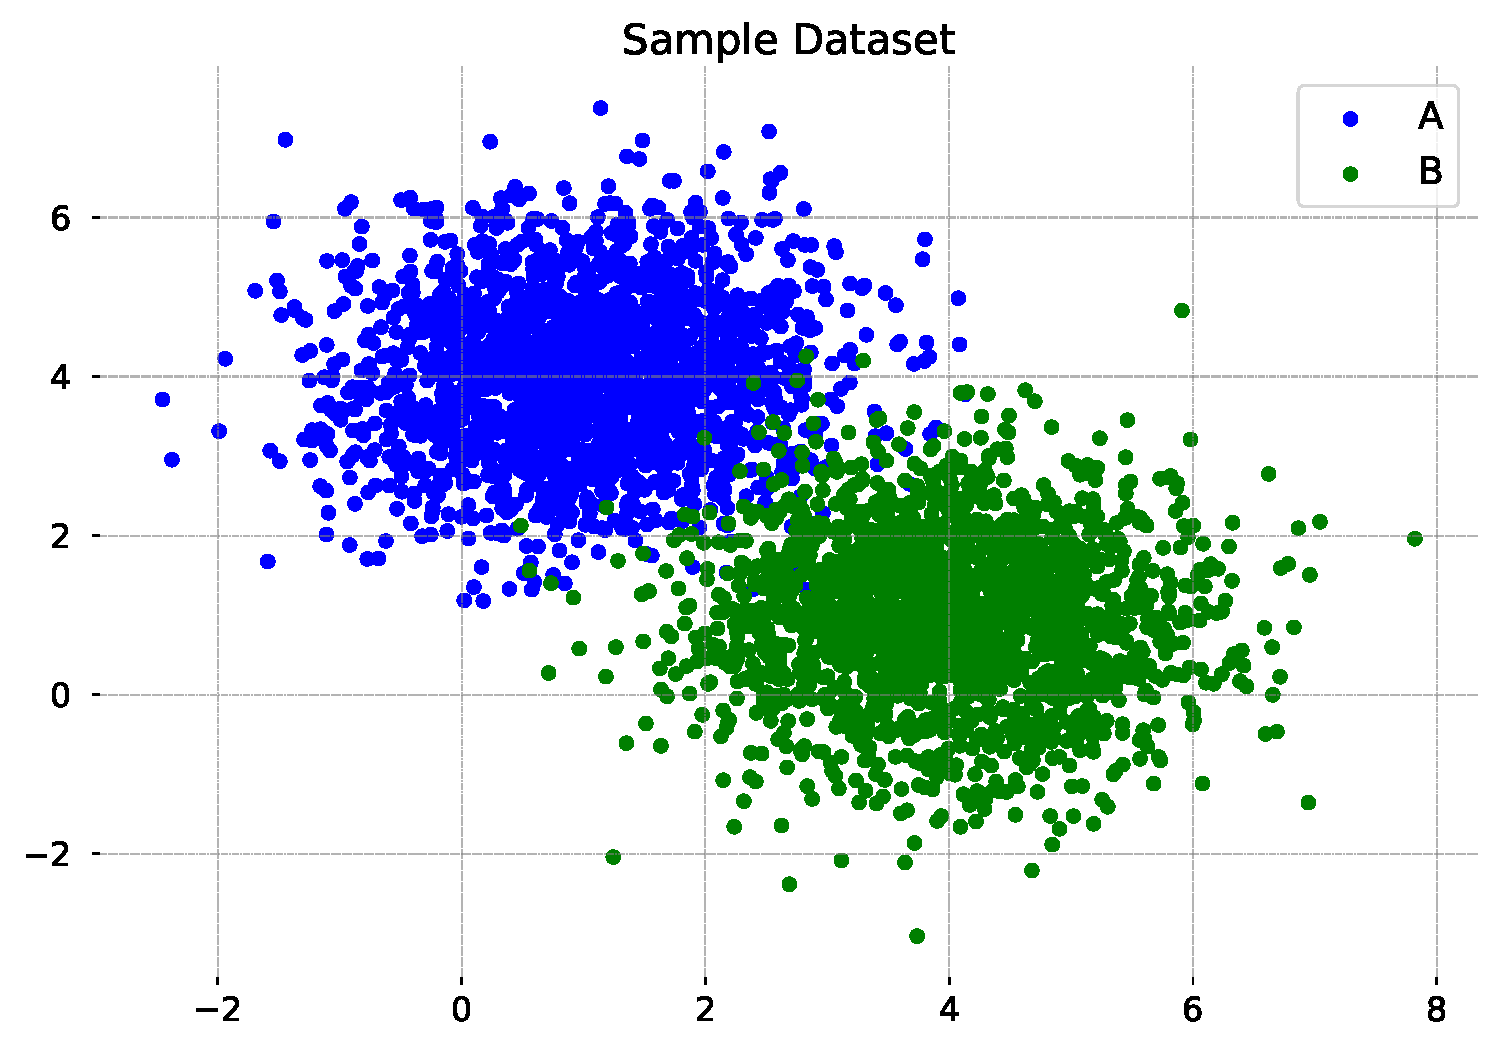
\includegraphics[width=0.95\linewidth]{c3_figures/sample_dataset.pdf}
%         \end{minipage}
%         \begin{minipage}{0.45\textwidth}
%             \centering
%             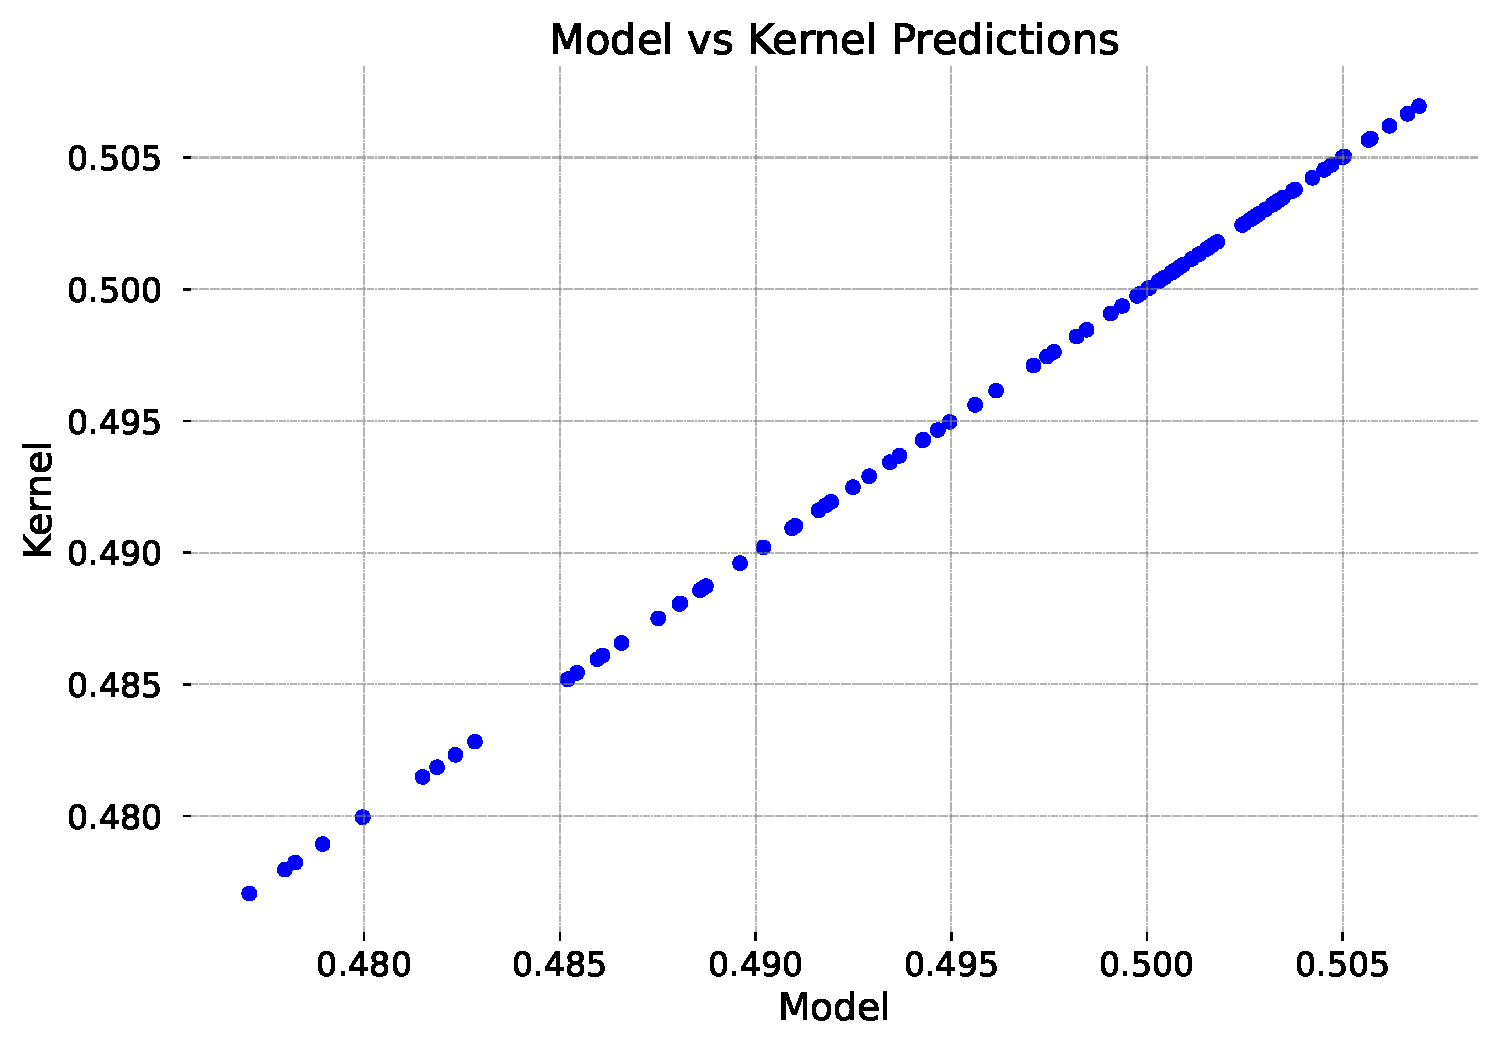
\includegraphics[width=0.95\linewidth]{c3_figures/model_kernel_predictions.pdf}
%         \end{minipage}
%         \caption{On the left is a 2d dataset of points sampled from gaussians with different means. Specifically, class A is normally distributed with $\mu = \left[1, 4\right]$ and $\sigma^2 = 1$ while class B is $\mu = \left[4, 1\right]$ and $\sigma^2 = 1$. 2000 data points were sampled for each class. These values were chosen arbitrarily to provide separation with a limited amount of overlap. On the right is the prediction similarity between the kernel and the original model. This demonstrates that our kernel formulation accurately represents the trained network.}
%         \label{fig:sample_data}
%     \end{figure}

% \subsection{Evaluating The Kernel}

%     Examples of the kernel values across 4 test points are shown in Figure \ref{fig:kernel}.
%     We are interested in how the kernel is learning and whether this kernel will allow out-of-distribution (OOD) detection.

%     \begin{figure}[!htb]
%         \centering
%         \begin{minipage}{0.45\textwidth}
%             \centering
%             % \begin{wrapfigure}{l}
%             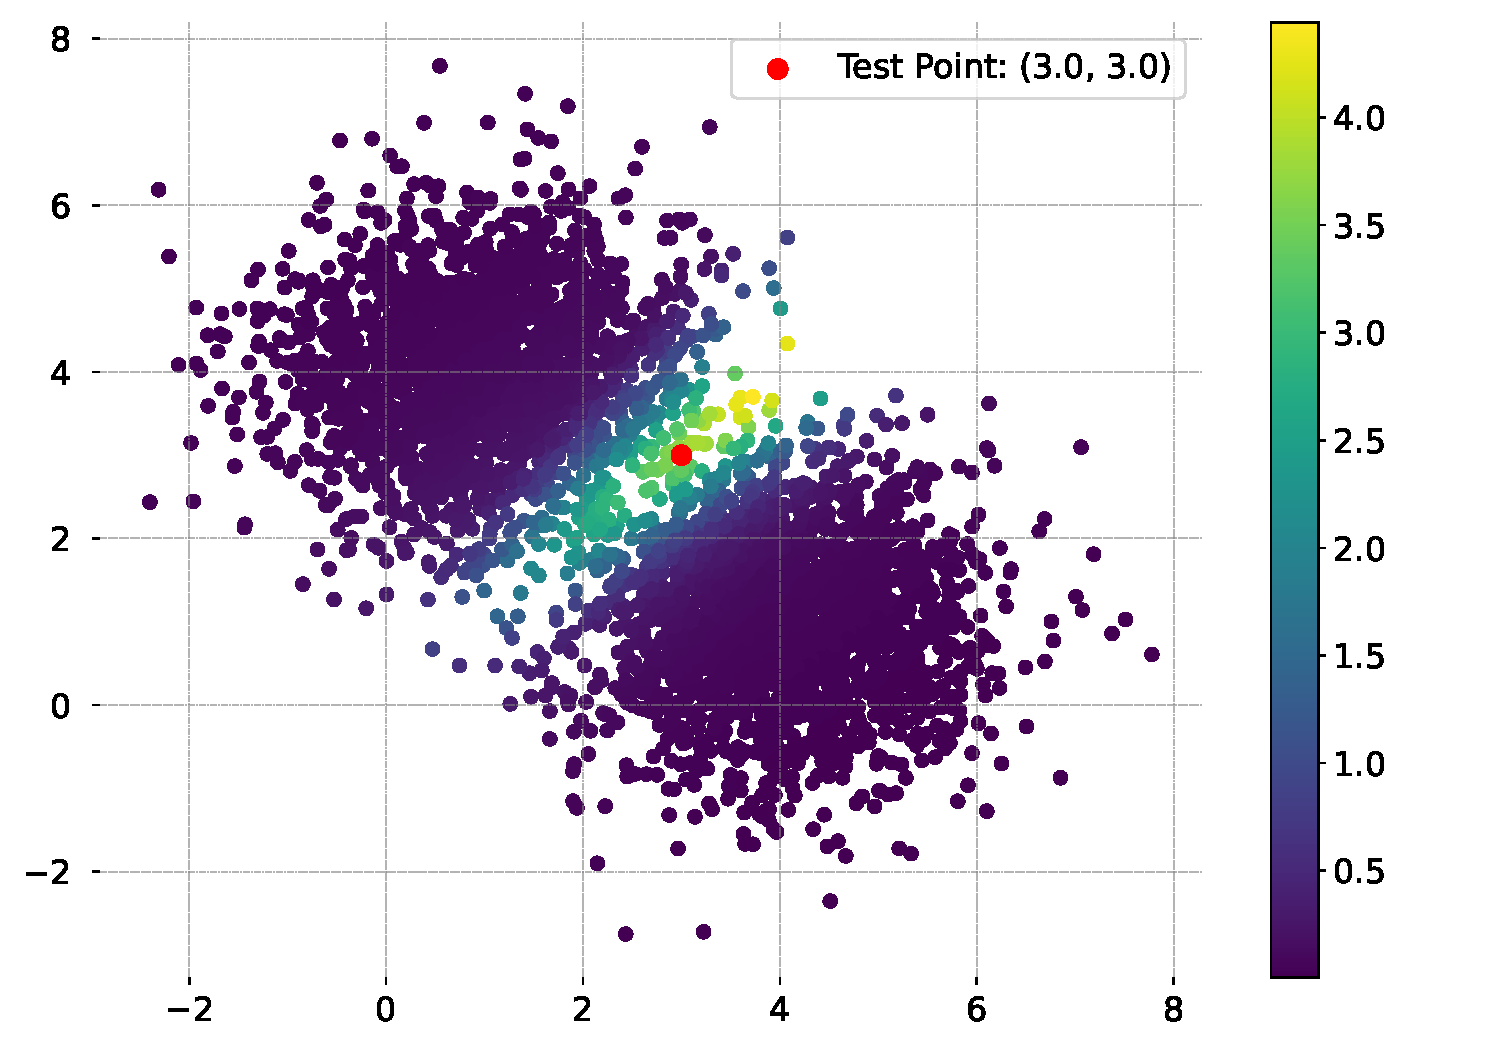
\includegraphics[width=0.95\linewidth]{c3_figures/in_distribution_uncertan.pdf}
%             % \caption{In Distribution}
%             % \end{wrapfigure}
%             % \captionof{figure}{Figure 1 is a figure}
%         \end{minipage}
%             \begin{minipage}{0.45\textwidth}
%                 \centering
%                 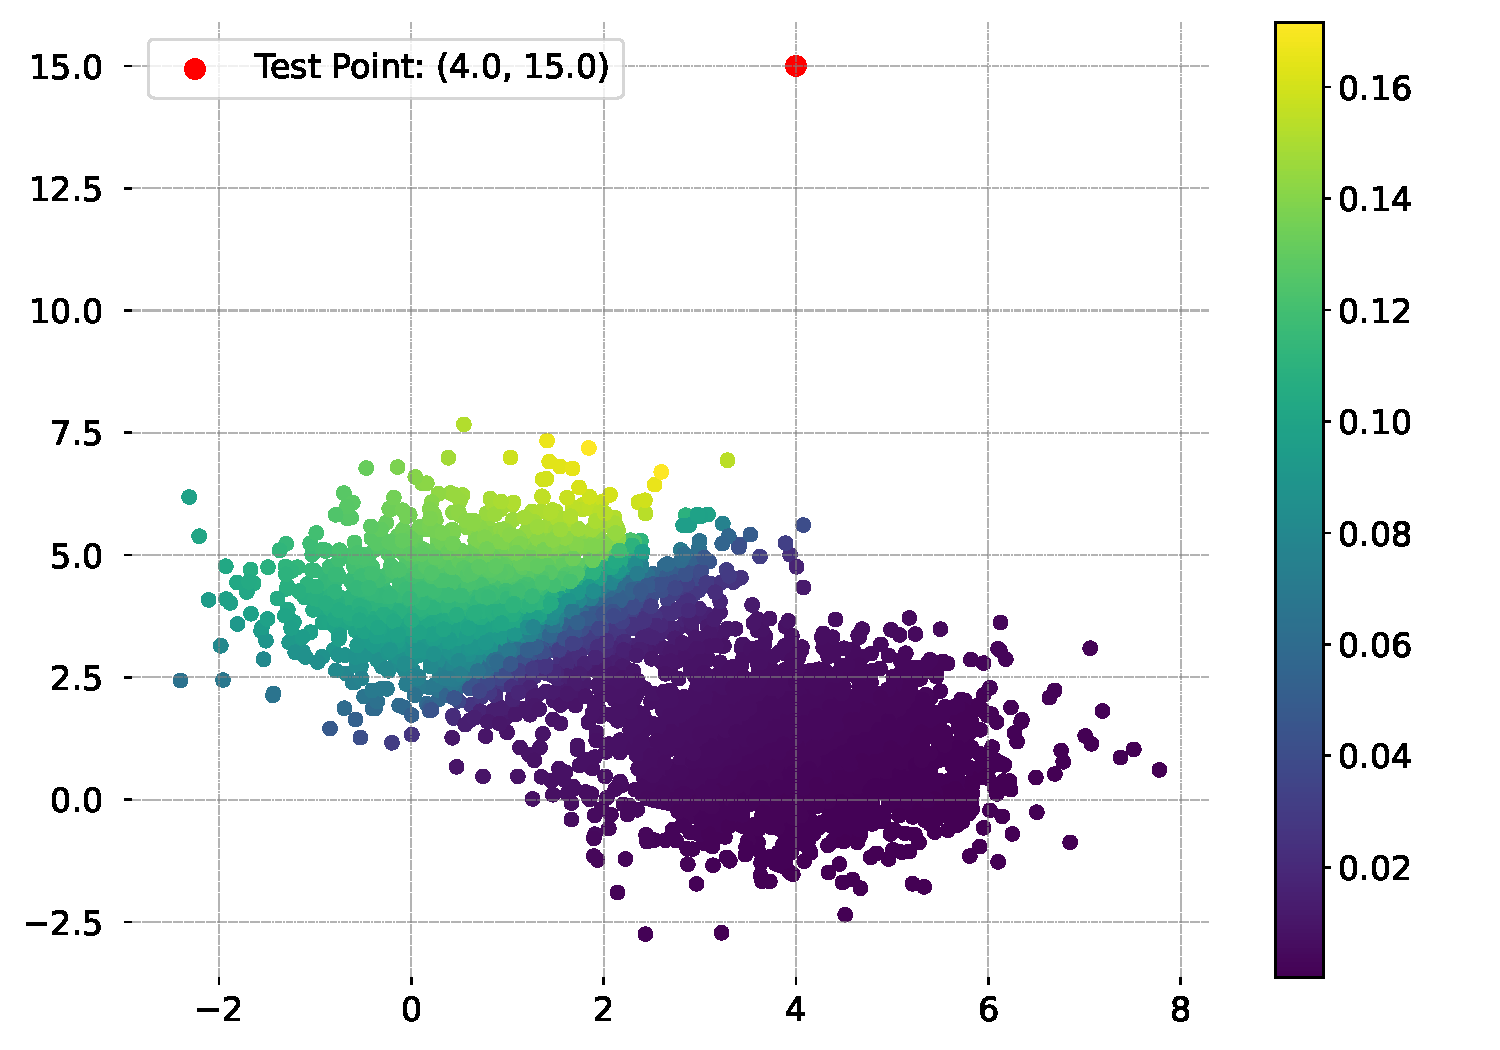
\includegraphics[width=0.95\linewidth]{c3_figures/ood_positive_2.pdf}
%                 % \captionof{figure}{Figure 1 is a figure}
%             \end{minipage}
%     %   \caption{Another figure caption.}
%     % \end{figure}

%     % \begin{figure}
%         \centering
%         \begin{minipage}{0.45\textwidth}
%             \centering
%             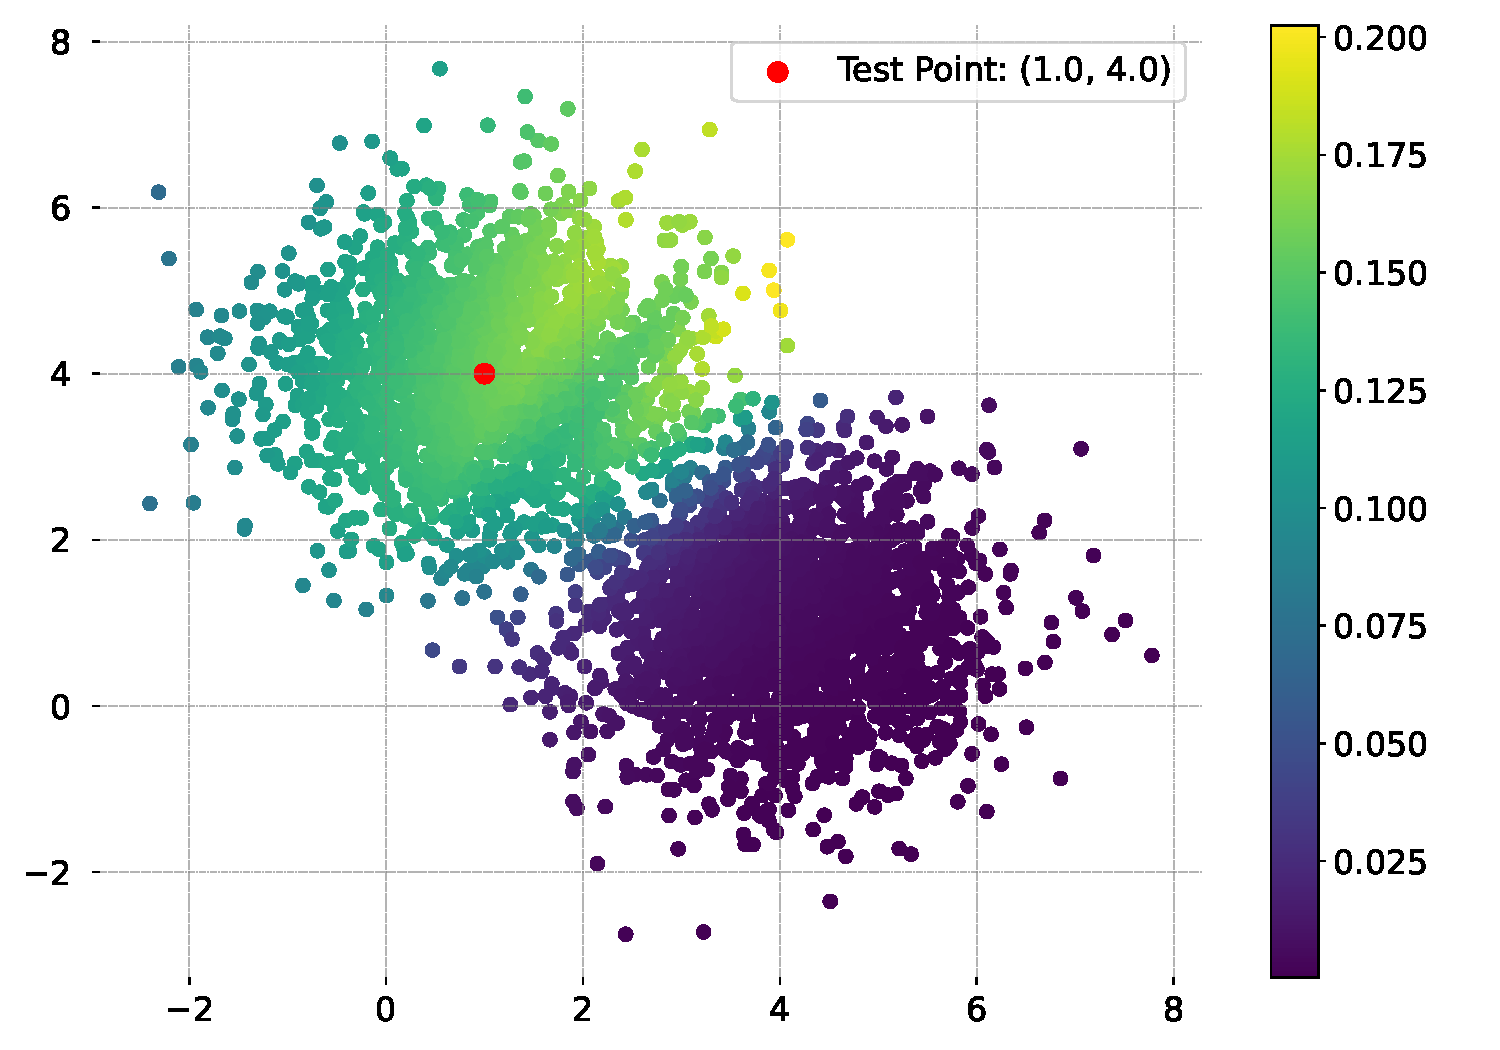
\includegraphics[width=0.95\linewidth]{c3_figures/in_distribution.pdf}
%             \captionsetup{labelformat=empty}
%             \captionof{figure}{In-Distribution}
%             \addtocounter{figure}{-1}
%             \end{minipage}
%             \begin{minipage}{0.45\textwidth}
%                 \centering
%                 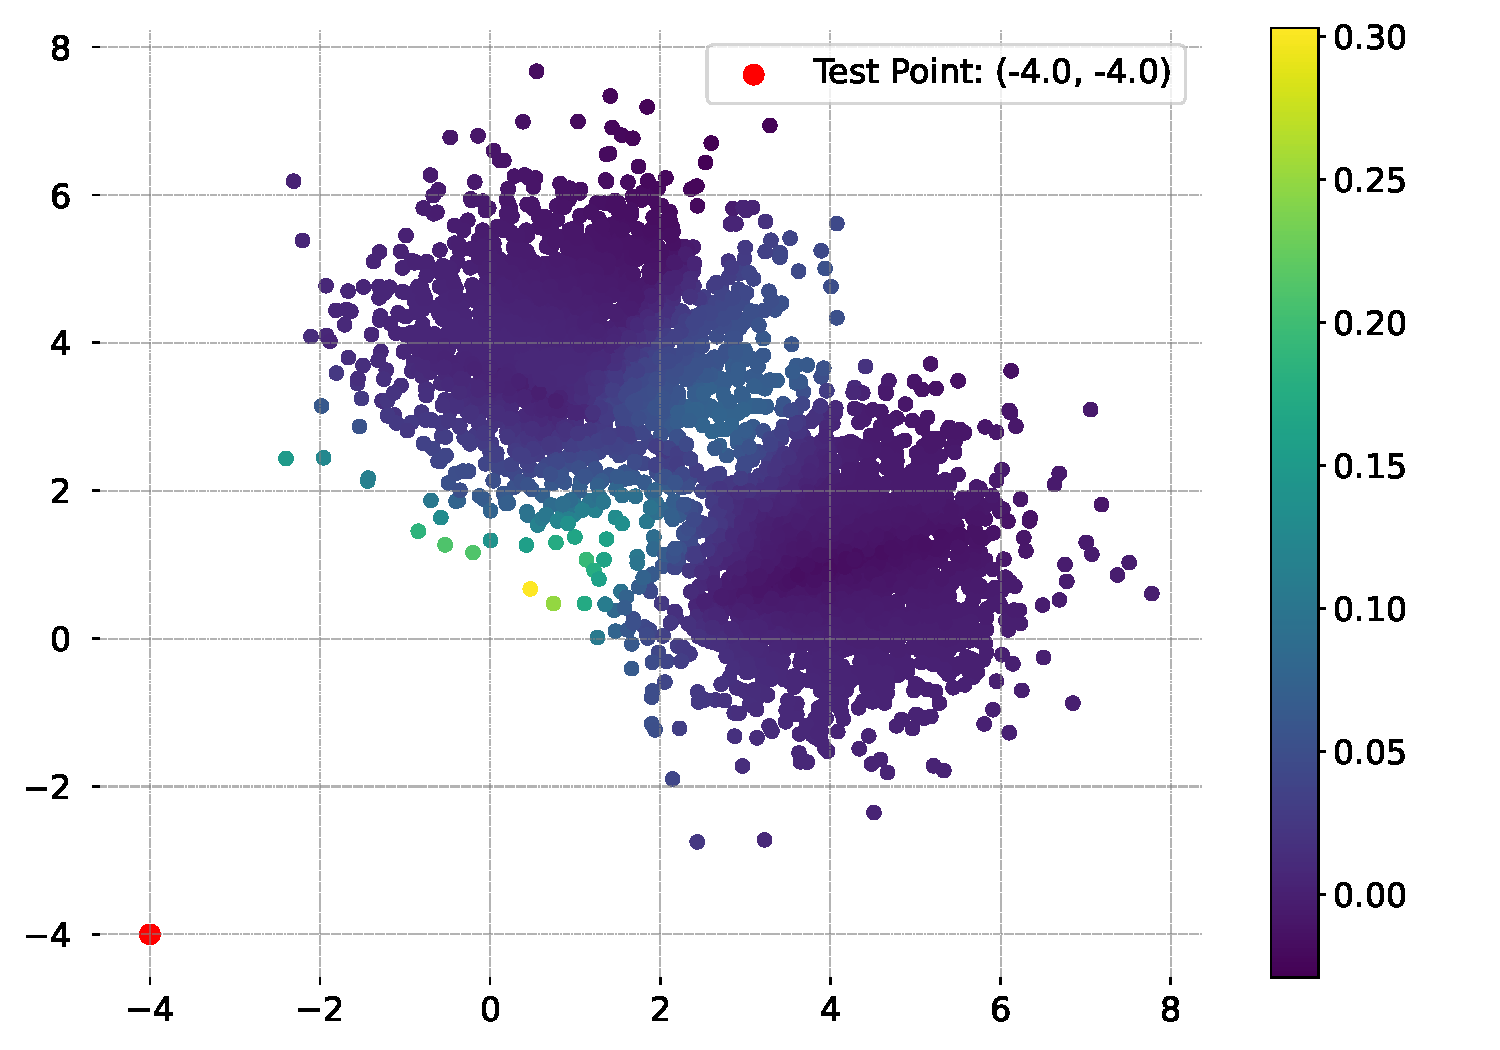
\includegraphics[width=0.95\linewidth]{c3_figures/ood.pdf}
%             \captionsetup{labelformat=empty}
%             \captionof{figure}{Out-Of-Distribution}
%             \addtocounter{figure}{-1}
%             \end{minipage}
%         \caption{Example of the kernel values on in-distribution and out-of-distribution (OOD) data. Left column shows samples which are in-distribution for our dataset. Right column row shows OOD samples.}
%         \label{fig:kernel}
%     \end{figure}
%     From these plots we see that the in-distribution samples have a significantly higher sum over kernel distances than the OOD examples. Of note is that the OOD detection is not perfect. For the test point $\left(4.0, 15.0\right)$ it still identifies a large portion of class A samples as being relatively close in kernel space. Despite this, both OOD examples shown are significantly lower in total kernel distance than the in-distribution samples. Further experiments will be required to better understand why some OOD regions are closer than others

% \subsection{Extending To Image Data}


%     We perform experiments on MNIST to demonstrate the applicability to image data. 
%     This kernel representation was generated for a two-layer fully connected ReLU Network with the cross-entropy loss-function, using Pytorch (citation). The model was trained using forward Euler (gradient descent) using gradients generated as a sum over all training data for each step. The state of the model was saved for every training step. In order to compute the per-training-point gradients needed for the kernel representation, the per-input jacobians are computed at execution time in the representation by loading the model for each training step $i$ , computing the jacobians for each training input to compute $\nabla_w \hat y_{w_s(0)}(x_i)$, and then repeating this procedure for 100 $t$ values between 0 and 1 in order to approximate $\int_0^1 \hat y_{w_s(t)}(x)$. Torch is not currently optimized to provide per-input jacobians or to provide jacobians for multiple weight states, so this procedure can be accelerated greatly by deeper integration with existing pytorch tools. 
    
%     We are able to see the agreement between the neural network and its kernel representation in  figure ~\ref{fig:agree}. In figure ~\ref{fig:near} we see that the function learned by the kernel does not directly mimic euclidean distance in the image space. Samples which are nearby in kernel space are not necessarily nearby in pixel space. The similarity metric learned is a direct explanation of how the neural network is making decisions.

%         \begin{figure}
%         \centering
%         \begin{minipage}{0.2\textwidth}
%             \centering
%             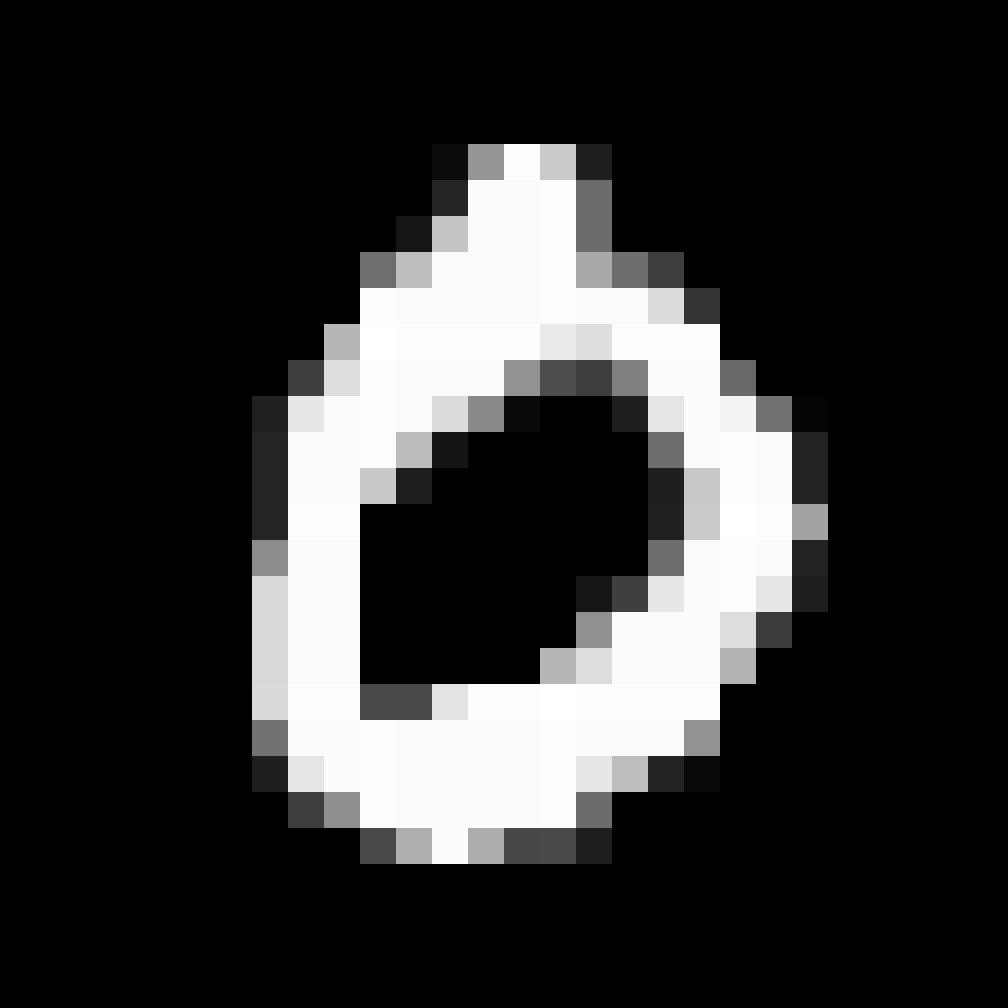
\includegraphics[width=0.95\linewidth]{c3_figures/samples/original_0.png}
%             % \captionof{figure}{Figure 1 is a figure}
%         \end{minipage}
%         \begin{minipage}{0.2\textwidth}
%             \centering
%             
\includegraphics[width=0.95\linewidth]{c3_figures/samples/8409_0.png}
%             % \captionof{figure}{Figure 1 is a figure}
%         \end{minipage}
%         \begin{minipage}{0.2\textwidth}
%             \centering
%             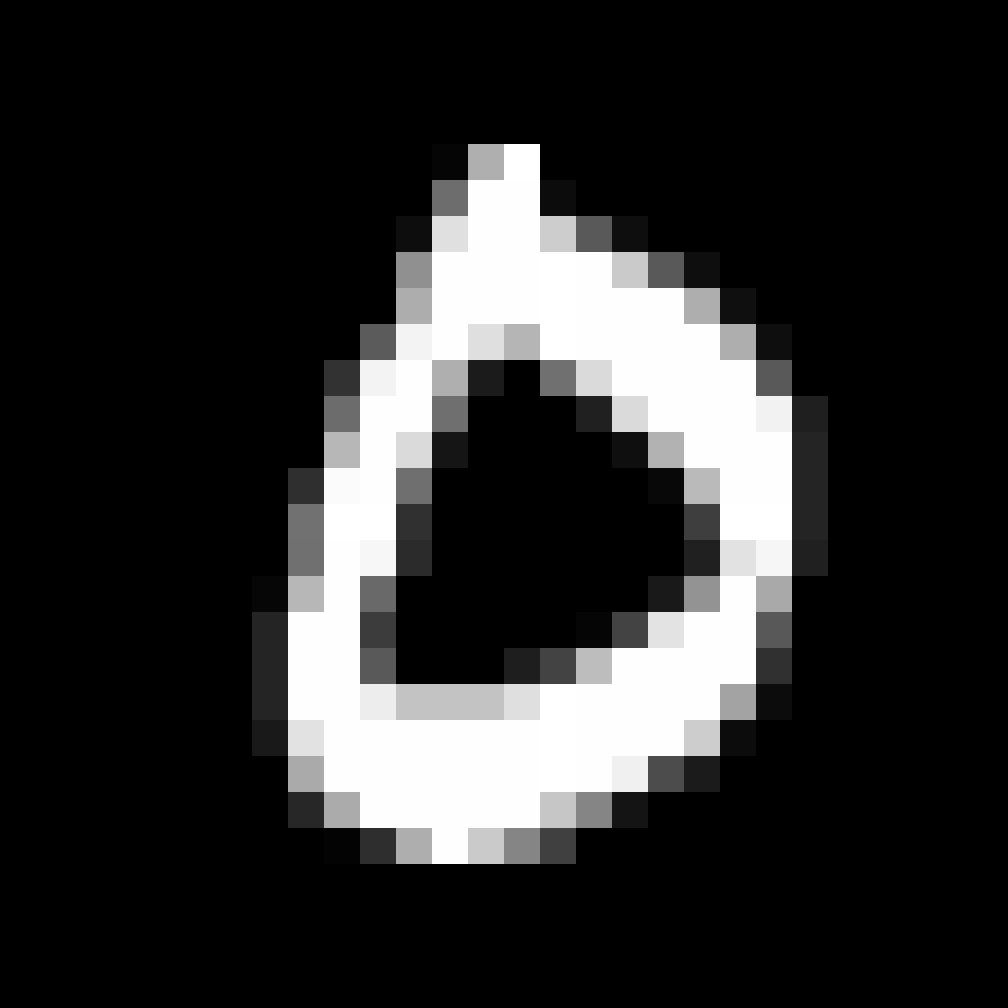
\includegraphics[width=0.95\linewidth]{c3_figures/samples/euclid_12516_0.png}
%             % \captionof{figure}{Figure 1 is a figure}
%         \end{minipage} \\
%         \vspace{.2cm}
%     %   \caption{Another figure caption.}
%         \centering
%         \begin{minipage}{0.2\textwidth}
%             \centering
%             
\includegraphics[width=0.95\linewidth]{c3_figures/samples/original_1.png}
%             \captionsetup{labelformat=empty}
%             \captionof{figure}{Original Image}            % \captionof{figure}{Figure 1 is a figure}
%             \addtocounter{figure}{-1}
%         \end{minipage}
%         \begin{minipage}{0.2\textwidth}
%             \centering
%             
\includegraphics[width=0.95\linewidth]{c3_figures/samples/322_0.png}
%             \captionsetup{labelformat=empty}
%             \captionof{figure}{Kernel Distance}            % \captionof{figure}{Figure 1 is a figure}
%             \addtocounter{figure}{-1}
%         \end{minipage}
%         \begin{minipage}{0.2\textwidth}
%             \centering
%             
\includegraphics[width=0.95\linewidth]{c3_figures/samples/euclid_3233_1.png}
%             % Pixel Distance
%             \captionsetup{labelformat=empty}
%             \captionof{figure}{Pixel Distance}
%             \addtocounter{figure}{-1}
%         \end{minipage}
%       \caption{Comparison between the nearest samples in kernel space and pixel space. From left to right in each column: Test set point, nearest sample in kernel space, nearest sample in pixel space using euclidean distance.}
%       \label{fig:near}
%     \end{figure}
    
%     % \begin{figure}
%     % \end{figure}

% \begin{figure}[!h]
% \centering
% 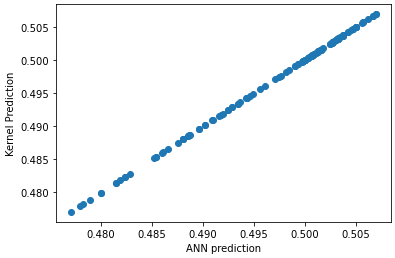
\includegraphics[width=8cm]{c3_figures/image.png}
% \caption{This plot shows output of the ANN versus output of the corresponding kernel representation for a set of test images from the MNIST dataset. We note the very strong agreement between the two outputs.}  
% \label{fig:agree}
% \end{figure}



% %I will leave it to michael to add any out-of-sample plots and plots related to $a_{i,s}$ weights and such. 

% \section{Discussion}

% The implications of a practical and finite kernel representation for neural networks are wide and profound. For most gradient trained models, there is a disconnect between the problem space (e.g. images) and the parameter space of a network. Parameters are intrinsically un-interpretable and much work has been spent building approximate mappings that convert model understanding back into the problem space in order to interpret features, sample importance, and other details (~\cite{simonyan2013deep}, ~\cite{lundberg2017unified}, and ~\cite{Selvaraju_2019}). A kernel is composed of a direct mapping from the problem space into parameter space. This mapping allows much deeper understanding of gradient trained models because the internal state of the method has an exact representation mapped from the problem space. Sample importance is produced directly by looking at the kernel and its corresponding weights per training input. 

% As stated in previous work ~\cite{domingos2020}, this representation has strong implications about the structure of gradient trained models and how they can understand the problems that they solve. Since the kernel weights in this representation are fixed derivatives with respect to the loss function $L$, $a_{i, s} = -\varepsilon  \dfrac{\partial L(\hat y_{w_s}(x_i),  y_i)}{\partial \hat y_i}$ nearly all of the information used by the network is represented by the kernel mapping function and inner product. Inner products are not just measures of distance, they also measure angle. In fact, figure \ref{fig:grad} shows that for a typical training example, the $L_2$ norm of the weights changes monotonically by only 20-30\% during training. This means that the "learning" of a gradient trained model is dominated by change in angle, which is predicted for kernel methods in high dimensions ~\cite{hardle2004nonparametric}.

% \begin{figure}[!h]
% \centering
% 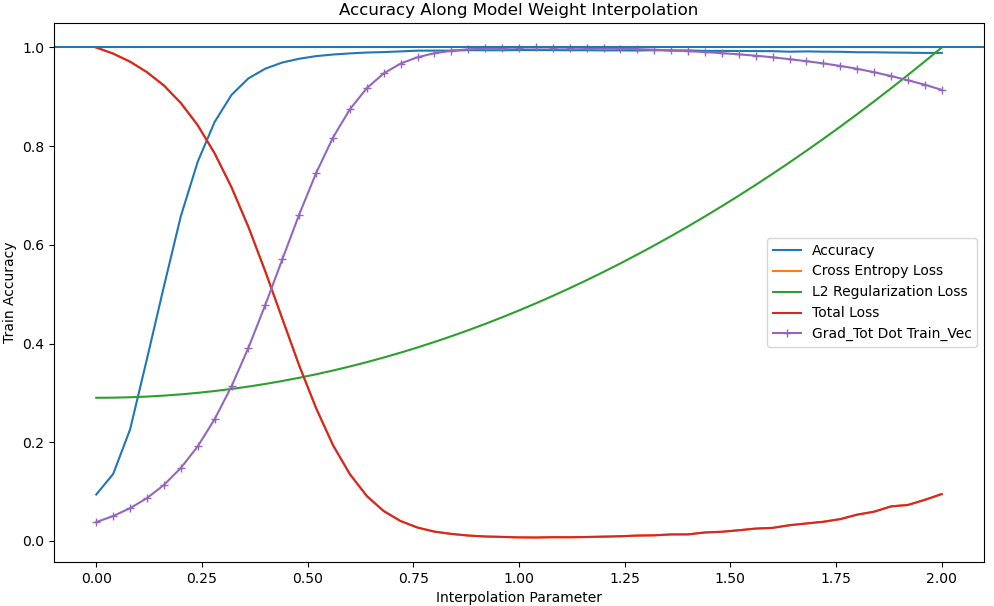
\includegraphics[width=12cm]{c3_figures/stab-n-201mnist-C32-100-100-10-0.001-0.0001-eval-mod_int_acc-trn.png}
% \caption{This plot shows a linear interpolation $w(t) = w_0 + t(w_{1} - w_0)$ of model parameters $w$ for a convolutional neural network $\hat y_w$ from their starting random state $w_0$ to their ending trained state $w_1$. The hatched blue line shows the dot product of the aggregated gradient over the training data $X$, $\langle \nabla_w \hat y_{w(t)}(X), (w_1 - w_0)/|w_1 - w_0| \rangle$. The other lines indicate accuracy (blue), total loss (red decreasing), and L2 Regularization (red increasing)}  
% \label{fig:grad}
% \end{figure}

% Perhaps the most significant advantage for gradient trained models of an exact kernel representation is that the combination of kernel and kernel weights provides a spatial representation of the model's understanding relative to the training data. In previous work (~\cite{gillette2022data} ~\cite{yousefzadeh2021deep} it has been shown that image classification can be represented by projection onto the convex hull of training data. This projection is computationally infeasible, but it provides a geometric gold-standard classifier. Since kernel methods provide a spatial representation of their prediction, this representation can be directly compared with convex hull projections. It also provides data through which we can infer the gradient model's understanding of the data spatially. 

% For kernel methods, this also represents a significant step. Despite their firm mathematical foundations, kernel methods have lost ground since the early 2000s due to the limitations of developing new kernels for complex high-dimensional problems ~\cite{NIPS2005_663772ea}. This opens up many modern problems to the powerful tools available to kernel methods. Of these, Gaussian Processes (GPs) may be the most exciting. Given our kernel function, we can generate covariance matrices for GP which will allow direct uncertainty measurement. This will allow much more significant analysis for out-of-distribution samples including adversarial attacks (~\cite{szegedy2013intriguing} ~\cite{ilyas2019adversarial}). 

% Gaussian processes are one of many research directions that naturally follow this work. It is worth noting that since the kernel from our representation can be either continuous or symmetric but not both (See remark ~\ref{rem:asym}), covariance matrices used in GPs will have slightly unusual properties that will reflect the divergence of the discrete training path from the smooth gradient flow. In the case of the asymmetric version of our representation, this asymmetry measures this divergence in a way that may be tractably explored using gaussian thermostats (~\cite{scherer2020kernel}, ~\cite{nose1990constant}). In addition to exploring GPs, it is natural to pursue more efficient computation of these representations by exploiting features of pytorch and incorporating the necessary integral computation with some codes that have been developed for NeuralODEs which require similar information (~\cite{bilovs2021neural}, ~\cite{neuralode2018})

% Another implication from this representation is the increased importance of models following their gradient flow during training. Since this derived kernel is either discontinuous or asymmetric depending on the neural network's training trajectory, developing training restrictions which satisfy equation ~\ref{eq:cond} may produce more useful kernels and have implications about the accuracy and generalizability of ANN models. This will provide a new motivation for such research separate from just the question of efficiency of training. Approaches in this direction may be found in control theory (~\cite{lin2020gradient}) and the neural ODE approach (~\cite{bilovs2021neural}, ~\cite{neuralode2018}). Also in this vein is the precise formulation of the divergence error from the discrete training path to the smooth gradient flow. Such a formulation should shed light on the dynamics of how such representations converge in performance under various step refinements. 

% \section{Acknowledgements}

% This research was funded by Los Alamos National Lab LDRD-DR XX9C UQ4ML (help with how to acknowledge this LDRD funding juston?) Thanks to Yen Ting Lin, Philip Hoskins, Keenan Eikenberry, and Craig Thompson for feedback on early iterations of this paper. 


% % \appendix
% % \section{Appendix}

% ex
% \subsection{The DPK is a Kernel}

% \ker*
% \begin{proof}
% We must show that the associated kernel matrix $K_{\text{DPK}} \in \mathbb{R}^{n\times n}$ defined for an arbitrary subset of data $\{x_i\}_{i=1}^M \subset X$ as $K_{\text{DPK},i,j} = \int_0^1\langle \phi_{s,t}(x_i), \phi_{s,t}(x_j)\rangle dt$ is both symmetric and positive semi-definite.

% Since the inner product on a Hilbert space $\langle \cdot, \cdot \rangle$ is symmetric and since the same mapping $\varphi$ is used on the left and right, $K_{\text{DPK}}$ is \textbf{symmetric}. 

% To see that $K_{\text{DPK}}$ is \textbf{Positive Semi-Definite}, let $f = (f_1, f_2, \dots, f_n)^\top \in \mathbb{R}^n$ be any vector. We need to show that $f^\top K_{\text{DPK}} f \geq 0$. We have

% \begin{align}
% f^\top K_{\text{DPK}} f &= \sum_{i=1}^n \sum_{j=1}^n f_i f_j \int_0^1 \langle \phi_{s,t}(x_i), \phi_{s,t}(x_j)\rangle dt \\
% &= \sum_{i=1}^n \sum_{j=1}^n f_i f_j \int_0^1 \langle \nabla_{w}\hat{y}_{w_s(t,x_i)}, \nabla{w}\hat{y}_{w_s(t,x_j)}\rangle dt \\
% &= \int_0^1 \sum_{i=1}^n \sum_{j=1}^n f_i f_j \langle \nabla_{w}\hat{y}_{w_s(t,x_i)}, \nabla_{w}\hat{y}_{w_s(t,x_j)}\rangle dt \\
% &= \int_0^1 \sum_{i=1}^n \sum_{j=1}^n  \langle f_i \nabla_{w}\hat{y}_{w_s(t,x_i)}, f_j \nabla_{w}\hat{y}_{w_s(t,x_j)}\rangle dt \\
% &= \int_0^1    \langle \sum_{i=1}^n f_i \nabla_{w}\hat{y}_{w_s(t,x_i)}, \sum_{j=1}^n f_j \nabla_{w}\hat{y}_{w_s(t,x_j)}\rangle dt \\
% & \text{Re-ordering the sums so that their indices match, we have}\\
% &= \int_0^1 \left\lVert \sum_{i=1}^n f_i \nabla_{w}\hat{y}_{w_s(t,x_i)}\right\rVert^2 dt \\
% &\geq 0,
% \end{align}

% Note that this reordering does not depend on the continuity of our mapping function $\phi_{s,t}(x_i)$.

% \end{proof}

% \textbf{Remark} In the case that our mapping function $\varphi$ is not symmetric, after re-ordering, we still yield something of the form:
% \begin{align}
% &= \int_0^1 \left\lVert \sum_{i=1}^n f_i \nabla_{w}\hat{y}_{w_s(t,x_i)}\right\rVert^2 dt \\
% \end{align}
% The natural asymmetric $\varphi$ is symmetric for every non-training point, so we can partition this sum. For the non-training points, we have symmetry, so for those points we yield exactly the $L^2$ metric. For the remaining points, if we can pick a Lipschitz constant $E$ along the entire gradient field, then if training steps are enough, then the integral and the discrete step side of the asymmetric kernel will necessarily have positive inner product. In practice, this Lipschitz constant will change during training and for appropriately chosen step size (smaller early in training, larger later in training) we can guarantee positive-definiteness. In particular this only needs to be checked for training points. 

% \subsection{The DPK is an Exact Representation}

% \ekr*
% \begin{proof}

% Let $\hat y_{w}$ be a differentiable function parameterized by parameters $w$ which is trained via $N$ forward Euler steps of fixed step size $\varepsilon$ on a training dataset $X$ with labels $ Y$, with initial parameters $w_0$ so that there is a constant $b$ such that for every $x$, $\hat y_{w_0}(x) = b$, and weights at each step ${w_s : 0 \leq s \leq N}$. Let $x \in X$ be arbitrary and within the domain of $\hat y_w$ for every $w$. For the final trained state of this model $\hat y_{w_N}$, let $y = \hat y_{w_N}(x)$. 

% For one step of training, we consider $y_s  = \hat y_{w_s}(x)$ and $y_{s+1} = \hat y_{w_{s+1}}(x)$. We wish to account for the change $y_{s+1} - y_s$ in terms of a gradient flow, so we must compute $\dfrac{\partial \hat y}{dt}$ for a continuously varying parameter $t$. Since $f$ is trained using forward Euler with a step size of $\varepsilon > 0$, this derivative is determined by a step of fixed size of the weights $w_s$ to $w_{s+1}$. We will parameterize this step in terms of the weights:

% \begin{align}
%     \dfrac{\partial w_s(t)}{dt} &= (w_{s+1} - w_s)\\   
%     \int \dfrac{\partial w_s(t)}{dt} dt &= \int (w_{s+1} - w_s)dt\\
%     w_s(t) &= w_s + t(w_{s+1} - w_s)\\
% \end{align}
% Since $f$ is being trained using forward Euler, we can write:
% \begin{align}
%     \dfrac{\partial w_s(t)}{dt} &= -\varepsilon \nabla_w L(\hat y_{w_s}(x_i), y_i) = -\varepsilon \sum_{j = 1}^{d} \dfrac{\partial L(\hat y_{w_s}(x_i),  y_i)}{\partial w_j} \label{eq10}
% \end{align}
% Applying chain rule and the above substitution, we can write
% \begin{align}
%     \dfrac{\partial \hat y}{dt} = \dfrac{d \hat y_{w_s(t)}}{dt} &= \sum_{j = 1}^{d} \dfrac{\partial \hat y}{\partial w_j} \dfrac{\partial w_j}{dt}\\
% &= \sum_{j = 1}^{d} \dfrac{\partial \hat y_{w_s(t)}(x)}{\partial w_j} \left(-\varepsilon \dfrac{\partial L(\hat y_{w_s}(X_T),  Y_T)}{\partial w_j}\right)\\
% &= \sum_{j = 1}^{d} \dfrac{\partial \hat y_{w_s(t)}(x)}{\partial w_j} \left(-\varepsilon \sum_{i = 1}^{M}\dfrac{\partial L(\hat y_{w_s}(x_i),  y_i)}{\partial \hat y_i}\dfrac{\partial \hat y_{w_s}(x_i)}{\partial w_j}\right)\\
% &= -\varepsilon \sum_{i = 1}^{M} \dfrac{\partial L(\hat y_{w_s}(x_i),  y_i)}{\partial \hat y_i} \sum_{j = 1}^{d} \dfrac{\partial \hat y_{w_s(t)}(x)}{\partial w_j}  \dfrac{\partial \hat y_{w_s}(x_i)}{\partial w_j}\\
% &= -\varepsilon \sum_{i = 1}^{M} \dfrac{\partial L(\hat y_{w_s}(x_i),  y_i)}{\partial \hat y_i}  \nabla_w \hat y_{w_s(t)}(x) \cdot \nabla_w \hat y_{w_s}(x_i)\\
% \end{align}
% Using the fundamental theorem of calculus, we can compute the change in the model's output over step $s$
% \begin{align}
%     y_{s+1} - y_s &= \int_0^1 -\varepsilon \sum_{i = 1}^{M} \dfrac{\partial L(\hat y_{w_s}(x_i),  y_i)}{\partial \hat y_i}  \nabla_w \hat y_{w_s(t)}(x) \cdot \nabla_w \hat y_{w_s}(x_i)dt\\
%  &=  -\varepsilon \sum_{i = 1}^{M} \dfrac{\partial L(\hat y_{w_s}(x_i),  y_i)}{\partial \hat y_i}  \left(\int_0^1\nabla_w \hat y_{w_s(t)}(x)dt\right) \cdot \nabla_w \hat y_{w_s}(x_i)\\
% \end{align}
% For all $N$ training steps, we have
% \begin{align}
% y_N &= b + \sum_{s=1}^N y_{s+1} - y_s\\
% y_N &= b + \sum_{s = 1}^N -\varepsilon \sum_{i = 1}^{M} \dfrac{\partial L(\hat y_{w_s}(x_i),  y_i)}{\partial \hat y_i}  \left(\int_0^1\nabla_w \hat y_{w_s(t)}(x)dt\right) \cdot \nabla_w \hat y_{w_s}(x_i)\\
% % &= \sum_{i = 1}^{M}\sum_{s = 1}^N -\varepsilon  \dfrac{\partial L(\hat y_{w_s}(x_i),  y_i)}{\partial \hat y_i}  \left(\int_0^1\nabla_w \hat y_{w_s(t)}(x)dt\right) \cdot \nabla_w \hat y_{w_s}(x_i)\\
% % &= \sum_{i = 1}^{M}\sum_{s = 1}^N -\varepsilon  \dfrac{\partial L(\hat y_{w_s}(x_i),  y_i)}{\partial \hat y_i}  \int_0^1\left\langle \nabla_w \hat y_{w_s(t)}(x), \nabla_w \hat y_{w_s}(x_i) \right\rangle dt\\ 
% &= b + \sum_{i = 1}^{M}\sum_{s = 1}^N -\varepsilon  \dfrac{\partial L(\hat y_{w_s}(x_i),  y_i)}{\partial \hat y_i}  \int_0^1\left\langle \nabla_w \hat y_{w_s(t,x)}(x), \nabla_w \hat y_{w_s(t,x_i)}(x_i) \right\rangle dt\\ 
% &= b + \sum_{i = 1}^{M}\sum_{s = 1}^N a_{i, s}  \int_0^1 \left\langle \phi_{s,t}(x), \phi_{s,t}(x_i)\right\rangle dt
% \end{align}
% Since an integral of a symmetric positive semi-definite function is still symmetric and positive-definie and likewise for discrete sums, this represention is a kernel method. 

% \end{proof}
% \subsection{When is an Ensemble of Kernel Machines itself a Kernel Machine?}
% Here we investigate when our derived ensemble of kernel machines composes to a single kernel machine.
% In order to show that a linear combination of kernels also equates to a kernel it is sufficient to show that $sign(a_{i,s}) = sign(a_{i,0})$ for all $a_{i,s}$. 
% In this case it is possible to let the sample weights of our final kernel machine equal $sign(a_{i,0})$.
% In order to show this, we impose some structure on the loss function and network.
% Here we show this is the case for binary crossentropy on a network with sigmoid activations on the logits.
% (TODO: More argument here using mercer's theorem. All positive linear combinations of kernels are kernels. There are cases where some negative coefficients are allowed but that's going to take a lot more thought. How do we extend this to say $aKa > 0$ for all $a$?)

% \begin{proof}

% \begin{align}
%     L(\hat y_i,  y_i) 
%     &= -  y_i \ln(\hat y_i) - (1 - y_i)\ln(1 - \hat y_i)\\
%     \dfrac{\partial L(\hat y_i,  y_i)}{\partial \hat y_i} &= \dfrac{y_i - \hat y_i}{(\hat y_i - 1) \hat y_i}
% \end{align}
% For a binary classification problem it is standard to have $y_i \in \{0, 1\}$ and using a sigmoid activation on the final layer we have $\hat y_i \in (0, 1)$. \\

% \begin{center}
    
% \begin{minipage}{0.45\textwidth}
% Assume $y_i = 0$.
% \begin{align}
%     \dfrac{\partial L(\hat y_i,  y_i)}{\partial \hat y_i} &= \dfrac{0 - \hat y_i}{(\hat y_i - 1) \hat y_i}\\
%     &= \dfrac{-1}{\hat y_i - 1}\\
%     &= \dfrac{1}{|\hat y_i - 1|}
% \end{align}
% The last equality relies on the fact that $\hat y_i < 1$.
% \begin{equation}
%     y_i = 0 \implies \dfrac{\partial L(\hat y_i,  y_i)}{\partial \hat y_i} > 0
% \end{equation}
% \end{minipage}
% \hspace{0.04\textwidth}
% \begin{minipage}{0.45\textwidth}
% Assume $y_i = 1$.
% \begin{align}
%     \dfrac{\partial L(\hat y_i,  y_i)}{\partial \hat y_i} &= \dfrac{1 - \hat y_i}{(\hat y_i - 1) \hat y_i}\\
%     &= \dfrac{1 - \hat y_i}{-(1-\hat y_i) \hat y_i}\\
%     &= -\dfrac{1}{\hat y_i}
% \end{align}
% Because $\hat y_i > 0$.
% \begin{equation}
%     y_i = 1 \implies \dfrac{\partial L(\hat y_i,  y_i)}{\partial \hat y_i} < 0
% \end{equation}
% \end{minipage}
% \end{center}

% This shows that the sign of the gradient of the loss function depends only on the label $y_i$, not on the predicted value of our model $\hat y_i$ and is constant through training. 
% Therefore:
% \begin{align}
%     y_S &= b - \varepsilon \sum_{i = 1}^{N}\sum_{s = 1}^S a_{i, s}  \int_0^1 \left\langle \phi_{s,t}(x), \phi_{s,t}(x_i)\right\rangle dt\\
%      &= b - \varepsilon \sum_{i = 1}^{N}sign(a_{i, 0}) \sum_{s = 1}^S |a_{i, s}| \int_0^1 \left\langle \phi_{s,t}(x), \phi_{s,t}(x_i)\right\rangle dt
% \end{align}
% This formulates a kernel machine where
% \begin{align}
% a_{i, 0} &= sign(\dfrac{\partial L(\hat y_{w_0}(x_i),  y_i)}{\partial \hat y_i}) \in \{-1, 1\} \\
% K(x, x_i) &= \sum_{s = 1}^S |a_{i, s}| \int_0^1 \left\langle \phi_{s,t}(x), \phi_{s,t}(x_i)\right\rangle dt \\
% \phi_{s,t}(x) &=  \nabla_w \hat y_{w_s(t,x)} (x)\\
% w_s(t,x) &= \begin{cases} w_s, x \in X_T\\ w_s(t), x \notin X_T \end{cases}\\
% b &= 0
% \end{align}
% \end{proof}


% This argument does not hold in the simple case of linear regression. 
% Assume our loss is instead squared error. Our labels are continuous on $\mathds{R}$ and our activation is the identity function.
% \begin{align}
%     L(\hat y_i,  y_i) 
%     &= (y_i - \hat y_{i, s})^2 \\
%     \dfrac{\partial L(\hat y_i,  y_i)}{\partial \hat y_i} &= 2(y_i- \hat y_{i, s})
% \end{align}

% This quantity is dependent on $\hat y_i$ and its sign is changing throughout training. (TODO: Make this more formal and rigorous)

% In order for 
% \begin{align}
%     \sum_{s=1}^S a_{i,s} \int_0^1 \langle \phi_{s,t}(x), \phi_{s,t}(x_i)\rangle dt
% \end{align}
% to be a kernel on its own, we need it to be a positive (or negative) definite operator. In the specific case of our practical path kernel, i.e. that in $K(x,x')$ if $x'$ happens to be equal to $x_i$, then:
% \begin{align}
%     &= \sum_{s=1}^S 2(y_i- \hat y_{i, s}) \int_0^1 \langle \phi_{s,t}(x), \phi_{s,t}(x_i)\rangle dt\\
%     &= \sum_{s=1}^S 2(y_i- \hat y_{i, s}) \int_0^1 \langle \nabla_w \hat y_{w_s(t))} (x), \nabla_w \hat y_{w_s(0)} (x_i)\rangle dt\\
%     &= \sum_{s=1}^S 2 \left(y_i \cdot \int_0^1 \langle \nabla_w \hat y_{w_s(t))} (x), \nabla_w \hat y_{w_s(0)} (x_i)\rangle dt - \hat y_{i, s} \int_0^1 \langle \nabla_w \hat y_{w_s(t))} (x), \nabla_w \hat y_{w_s(0)} (x_i)\rangle dt \right)\\
%     &= \sum_{s=1}^S 2 \left(y_i \cdot \int_0^1 \langle \nabla_w \hat y_{w_s(t))} (x), \nabla_w \hat y_{w_s(0)} (x_i)\rangle dt -  \int_0^1 \langle \nabla_w \hat y_{w_s(t))} (x), \hat y_{i, s} \nabla_w \hat y_{w_s(0)} (x_i)\rangle dt \right)\\
%     &= \sum_{s=1}^S 2 \left(y_i \cdot \int_0^1 \langle \nabla_w \hat y_{w_s(t))} (x), \nabla_w \hat y_{w_s(0)} (x_i)\rangle dt -  \int_0^1 \langle \nabla_w \hat y_{w_s(t))} (x), \dfrac{1}{2}\nabla_w (\hat y_{w_s(0)} (x_i))^2\rangle dt \right)\\
% \end{align}
% Otherwise, we get the usual 
% \begin{align}
%         &= \sum_{s=1}^S 2(y_i- \hat y_{i, s}) \int_0^1 \langle \nabla_w \hat y_{w_s(t,x))} (x), \nabla_w \hat y_{w_s(t,x)} (x')\rangle dt\\
% \end{align}
% The question is two fold. One, in general theory (i.e. the lower example), can we contrive two pairs $(x_1,x'_1)$ and $(x_2,x'_2)$ that don't necessarily need to be training or test images for which this sum is positive for $1$ and negative for $2$. Second, in the case that we are always comparing against training images, do we get something more predictable since there is greater dependence on $x_i$ and we get the above way of re-writing  using the gradient of the square of $\hat y(x_i)$. 


% \subsection{Multi-Class Case}

% There are two ways of treating our loss function $L$ for a number of classes (or number of output activations) $K$:
% \begin{align}
%     \text{Case 1: } L &: \mathbb{R}^K \to \mathbb{R}\\
%     \text{Case 2: } L &: \mathbb{R}^K \to \mathbb{R}^K\\
% \end{align}

% \subsubsection{Case 1 Scalar Loss}

% Let $L : \mathbb{R}^K \to \mathbb{R}$. We will be using the chain rule $D (g \circ f) (x) = Dg(f(x))Df(x)$. 

% Let $\hat y$ be a vector valued function so that $\hat y : \mathbb{R}^D \to \mathbb{R}^K$  satisfying the conditions from [representation theorem above] with $x \in \mathbb{R}^D$ and $y_i \in \mathbb{R}^K$ for every $i$. We note that $\dfrac{\partial \hat y}{\partial t}$ is a column and has shape $Kx1$ and our first chain rule can be done the old fashioned way on each row of that column:
% \begin{align}
%     \dfrac{\partial \hat y}{\partial t} &= \sum_{j=1}^M \dfrac{\partial \hat y(x)}{\partial w_j} \dfrac{\partial w_j}{\partial t}\\
%     &= -\varepsilon \sum_{j=1}^M \dfrac{\partial \hat y(x)}{\partial w_j} \sum_{i=1}^N \dfrac{\partial L(\hat y(x_i), y_i)}{\partial w_j}\\
%     &\text{Apply chain rule}\\
%     &= -\varepsilon \sum_{j=1}^M \dfrac{\partial \hat y(x)}{\partial w_j} \sum_{i=1}^N \dfrac{\partial L(\hat y(x_i), y_i)}{\partial \hat y}\dfrac{\partial \hat y(x_i)}{\partial w_j}\\
%     &\text{Let}\\
%     A &= \dfrac{\partial \hat y(x)}{\partial w_j} \in \mathbb{R}^{K \times 1}\\
%     B &= \dfrac{\partial L(\hat y(x_i), y_i)}{\partial \hat y} \in \mathbb{R}^{1 \times K}\\
%     C &= \dfrac{\partial \hat y(x_i)}{\partial w_j} \in \mathbb{R}^{K \times 1}
% \end{align}
% We have a matrix multiplication $ABC$ and we wish to swap the order so somehow we can pull $B$ out, leaving $A$ and $C$ to compose our product for the representation. Since $BC \in \mathbb{R}$, we have $(BC) = (BC)^T$ and we can write
% \begin{align}
%     (ABC)^T &= (BC)^TA^T = BCA^T\\
%     ABC &= (BCA^T)^T
% \end{align}
% Note: This condition needs to be checked carefully for other formulations so that we can re-order the product as follows:
% \begin{align}
%         &= -\varepsilon \sum_{j=1}^M  \sum_{i=1}^N \left(\dfrac{\partial L(\hat y(x_i), y_i)}{\partial \hat y} 
%         \dfrac{\partial \hat y(x_i)}{\partial w_j} \left(\dfrac{\partial \hat y(x)}{\partial  w_j}\right)^T\right)^T
%         \\
%     &= -\varepsilon \sum_{i=1}^N \left(\dfrac{\partial L(\hat y(x_i), y_i)}{\partial \hat y} 
%     \sum_{j=1}^M \dfrac{\partial \hat y(x_i)}{\partial w_j} \left(\dfrac{\partial \hat y(x)}{\partial w_j}\right)^T\right)^T\\        
% \end{align}
% Note, now that we are summing over $j$, so we can write this as an inner product on $j$ with the $\nabla$ operator which in this case is computing the jacobian of $\hat y$ along the dimensions of class (index k) and weight (index j). We can define 
% \begin{align}
%     (\nabla \hat y(x))_{k,j} &= \dfrac{\partial \hat y_{k}(x)}{\partial w_j}\\
%     &= -\varepsilon \sum_{i=1}^N \left(\dfrac{\partial L(\hat y(x_i), y_i)}{\partial \hat y} 
%      \nabla \hat y(x_i) (\nabla \hat y(x))^T\right)^T\\    
% \end{align}
% We note that the dimensions of each of these matrices in order are $[1,K]$, $[K,M]$, and $[M,K]$ which will yield a matrix of dimension $[1, K]$ i.e. a row vector which we then transpose to get back a column of shape $[K, 1]$

% \subsection{Multi Class Case}


% In the case where $\hat y$ is a vector we denote the data index by the superscript $y^{[i]}$ and the vector component by the subscript $y_k$.

% query point may need to know about other class gradients than the target class. 

% k by k

% yen ting's approach is needed because we are making some assumption about the model that allows us to measure the query change along a linear path. 

% The negative log likelyhood function where $y$ and $\hat y$ are vectors.
% \begin{align}
%     NLL(y, \hat y) = \sum_k^{K} -y_k \ln(\hat y_k)
% \end{align}

% \begin{align}
%     \dfrac{\partial \left[ \hat y_0 ... y_k \right]}{dt} &= \sum_{j=1}^M \dfrac{\partial \left[\hat y_0 ... \hat y_k \right]}{\partial w_j} \dfrac{\partial w_j}{dt}\\
%     &= \sum_{j=1}^M \dfrac{\partial \left[\hat y_0 ... \hat y_k \right]}{\partial w_j} \left( -\varepsilon \sum_{i = 1}^N \dfrac{\partial L(\hat y^{[i]}, y^{[i]})}{\partial w_j} \right)\\
%     &= \sum_{j=1}^M \dfrac{\partial \left[\hat y_0 ... \hat y_k \right]}{\partial w_j} \left( -\varepsilon \sum_{i = 1}^N \dfrac{\partial L(\hat y^{[i]}, y^{[i]})}{\partial \left[ \hat y^{[i]}_{0} ... \hat y^{[i]}_{k} \right]} \dfrac{\partial \left[ \hat y^{[i]}_{0} ... \hat y^{[i]}_{k} \right]}{\partial w_j} \right)\\
%     &=  -\varepsilon \sum_{i = 1}^N \dfrac{\partial L(\hat y^{[i]}, y^{[i]})}{\partial \left[ \hat y^{[i]}_{0} ... \hat y^{[i]}_{k} \right]} \sum_{j=1}^M  \dfrac{\partial \left[\hat y_0 ... \hat y_k \right]}{\partial w_j} \dfrac{\partial \left[ \hat y^{[i]}_{0} ... \hat y^{[i]}_{k} \right]}{\partial w_j} 
% \end{align}

% Now we use the fact that L is CCE
% \begin{align}
%     \dfrac{\partial L(\hat y^{[i]}, y^{[i]})}{\partial y^{[i]}_k} &= \begin{cases} 0, k \not = y^{[i]}\\ -1 \end{cases}
% \end{align}

% \begin{align}
%     \dfrac{\partial \hat y_k}{dt} &=  -\varepsilon \sum_{i = 1}^N 1 \sum_{j=1}^M  \dfrac{\partial \left[\hat y_0 ... \hat y_k \right]}{\partial w_j} \dfrac{\partial \left[ \hat y^{[i]}_{0} ... \hat y^{[i]}_{k} \right]}{\partial w_j} 
% \end{align}

% \begin{align}
%     y_0 +  \left[ \dfrac{\partial L(\hat y^{[i]}, y^{[i]})}{\partial y^{[i]}_0} \sum_{j=1}^M \dfrac{\partial f(x_i)_0}{\partial w_j} \cdot\dfrac{\partial f(x)_0}{\partial w_j}, \dfrac{\partial L(\hat y^{[i]}, y^{[i]})}{\partial y^{[i]}_1} \sum_{j=1}^M \dfrac{\partial f(x_i)_1}{\partial w_j} \cdot\dfrac{\partial f(x)_1}{\partial w_j} \right]
% \end{align}

% % \begin{align}
% % y_N &= b + \sum_{s=1}^N y_{s+1} - y_s\\
% %     &= b + \sum_{i = 1}^{M}\sum_{s = 1}^N -\varepsilon  \dfrac{\partial L(\hat y_{w_s}(x_i),  y_i)}{\partial \hat y_i}  \int_0^1\left\langle \nabla_w \hat y_{w_s(t,x)}(x), \nabla_w \hat y_{w_s(t,x_i)}(x_i) \right\rangle dt
% % \end{align}


% \section{Neural Networks are Gaussian Processes}
% With Dropout on, the interpolant from one class to another will go into a variety of other classes. If you make a histogram of the locations where these boundary crossings occur, that will show a gaussian. 

% insert figure(s)

% \section{prove path kernel result in context of differential flow of
% gradients on neural network. using forward euler approx of grad flow. }

% \section{** look for sample in weight space and look for gradients}
%   that are pointing toward the final point versus wanting a different
%   direction. Then dot product those with the training direction. 

% \section{training gradients are smooth}
% \section{robust network types : regularized, michael's pca, Soft Nearest Neighbor Loss (SNNL) and
% adversarially trained. }
% \section{high dimensional arcs are very similar to chords}
% \section{linear interpolated model parameters from random to trained
% state yield robust models}
% \subsection{For Mnist Inner Products in weight space matter more than
% distances} -- does this generalize to ImNet?
% \section{define robustness in terms of skew versus orthogonal}
% \section{define robustness in terms of attack perturbation magnitude}
